\documentclass[10pt, UKenglish]{beamer}
\usepackage{babel}
\usepackage[utf8]{inputenc}  
\usepackage{geometry}
\usepackage[customcolors]{hf-tikz}
\usepackage[T1]{fontenc}   
\usepackage{tcolorbox}
\usepackage{siunitx}
\usepackage{hyperref}
\usepackage{bookmark}
\usepackage{marvosym}
\usepackage{tikz}
\usepackage{tikz-qtree}
\usepackage{cancel}
\usepackage{todonotes}
\useoutertheme[subsection=false]{smoothbars}
\DeclareSIUnit[number-unit-product = {}]{\inchQ}{\textquotedbl}
\usepackage{amsmath}
\usepackage{amssymb}
\newcommand\hmmax{0} % default 3
% \newcommand\bmmax{0} % default 4
\usepackage{bm} 
\DeclareSIUnit[number-unit-product = {\thinspace}]{\inch}{in}
\usetheme[menuwidth={0.3\paperwidth}]{erlangen}
\usepackage{multicol}
\usepackage{charter}
\setbeamercovered{transparent=20}
\setbeamertemplate{navigation symbols}{}
\sisetup{separate-uncertainty = true}
\usepackage[version=4]{mhchem}
\usepackage{tikz}
\usepackage{hepnames}
\usepackage{soul}
\usepackage{color}
\usepackage{thesis_defs}
\usepackage{subcaption}
\usepackage{xcolor}
\usepackage{enumitem}
\setlist[enumerate]{labelindent=10pt,style=multiline,leftmargin=2.5cm}
\setlist[itemize]{font=$\bullet$\scshape\bfseries}

\usepackage[backend=biber]{biblatex}
\bibliography{bibliography.bib}

\graphicspath{%
  {./feynman_diagrams/}%
  {./figures_theory/}%
  {./figures_simple/}%
  {./figures_misc/}%
  {./app1/}%
  {./app2/}%
  {./app3/}%
}


\definecolor{color1}{RGB}{33,217,217}
\definecolor{color2}{RGB}{7,61,111}

\newcommand{\lr}{\mathcal{lr}}


\newcounter{totavalue}
\newcounter{parvalue}

\def\aux{1}
\def\radius{9pt}
\def\step{4pt}
\usepackage[absolute,overlay]{textpos}


\newcommand\circcounter{%
\ifnum\inserttotalframenumber<2\relax
\else
  \setcounter{totavalue}{\inserttotalframenumber}
  \setcounter{parvalue}{\insertframenumber}
  \ifnum\inserttotalframenumber>45\relax
    \renewcommand\step{0pt}
  \fi%
  \pgfmathsetmacro{\aux}{360/25}
  \begin{tikzpicture}[remember picture,overlay, rotate=90+\aux]
  \foreach \i in {0,1,...,25}
    \fill[logo_blue] 
      (0,0) -- (-\i*\aux:\radius) arc  (-\i*\aux:-(\i+1)*\aux+\step:\radius) -- cycle;
  \foreach \i in {1,...,\insertframenumber}
    \fill[logo_grey] 
      (0,0) -- (-\i*\aux:\radius) arc  (-\i*\aux:-(\i+1)*\aux+\step:\radius) -- cycle;
  \fill[white] circle (\radius/1.3);
  \node at (0,0) {\small\insertframenumber}; 
  \end{tikzpicture}%
\fi%
}


\usepackage{eso-pic,picture}



\begin{document} 

\title[Bachelorvortrag]{Categorical Neural Networks}
\subtitle{1st of September 2021}
\author{Christian Kirfel}
%\institute{Universtität Bonn}
        



\begin{frame}[plain]
\vspace{0.0cm}
  \titlepage
      \AddToShipoutPictureFG*{%
    \AtPageUpperLeft{%
      \put(8.7cm,-9.6cm){

\includegraphics[scale=0.03]{original_logo.jpg}
\makebox(0,0)[lt]{}%
      }%
    }%
  }%
    \AddToShipoutPictureFG*{%
    \AtPageUpperLeft{%
      \put(0.0cm,-9.6cm){
%\includegraphics[scale=0.17]{atlas_gay.png}
%
\includegraphics[scale=0.17]{ATLAS-Logo-Ref-RGB-H_0.jpg}
\makebox(0,0)[lt]{}%
      }%
    }%
  }%
\end{frame}
\addtobeamertemplate{navigation symbols}{\vspace*{0.8cm}\hfill\circcounter\hspace*{0.7cm}}

\section{Neural Networks}
\begin{frame}{Neural Networks - Processing information}
\begin{tabular}{p{5cm}|p{5cm}}
    \begin{figure}
    	
\includegraphics[scale = 0.09]{brain}
    \end{figure}
    & 
    \begin{figure}
    	
\includegraphics[scale = 1.4]{machine}
    \end{figure} \\
  \multicolumn{1}{c|}{Humam senses} & \multicolumn{1}{c}{Input variables} \\
    \begin{itemize}
        \item Extraction of relevant info
        \item Impossible for machines
    \end{itemize}
    & 
    \begin{itemize}
      \item Preprocessed by user
      \item {e.g.} kinematic variables
    \end{itemize} \\
\multicolumn{1}{c|}{Human brain} & \multicolumn{1}{c}{Net of nodes} \\
    \begin{itemize}
        \item Web of neuron cells
        \item Input from surrounding cells
        \item Single combination $\rightarrow$ action
    \end{itemize}
    & 
    \begin{itemize}
      \item Nodes = simple processors
      \item Connected by linear function
      \item Combination forms non-linear model
    \end{itemize} 
 \end{tabular}
\end{frame}


\begin{frame}{Neural network structure}
\begin{figure}
\centering
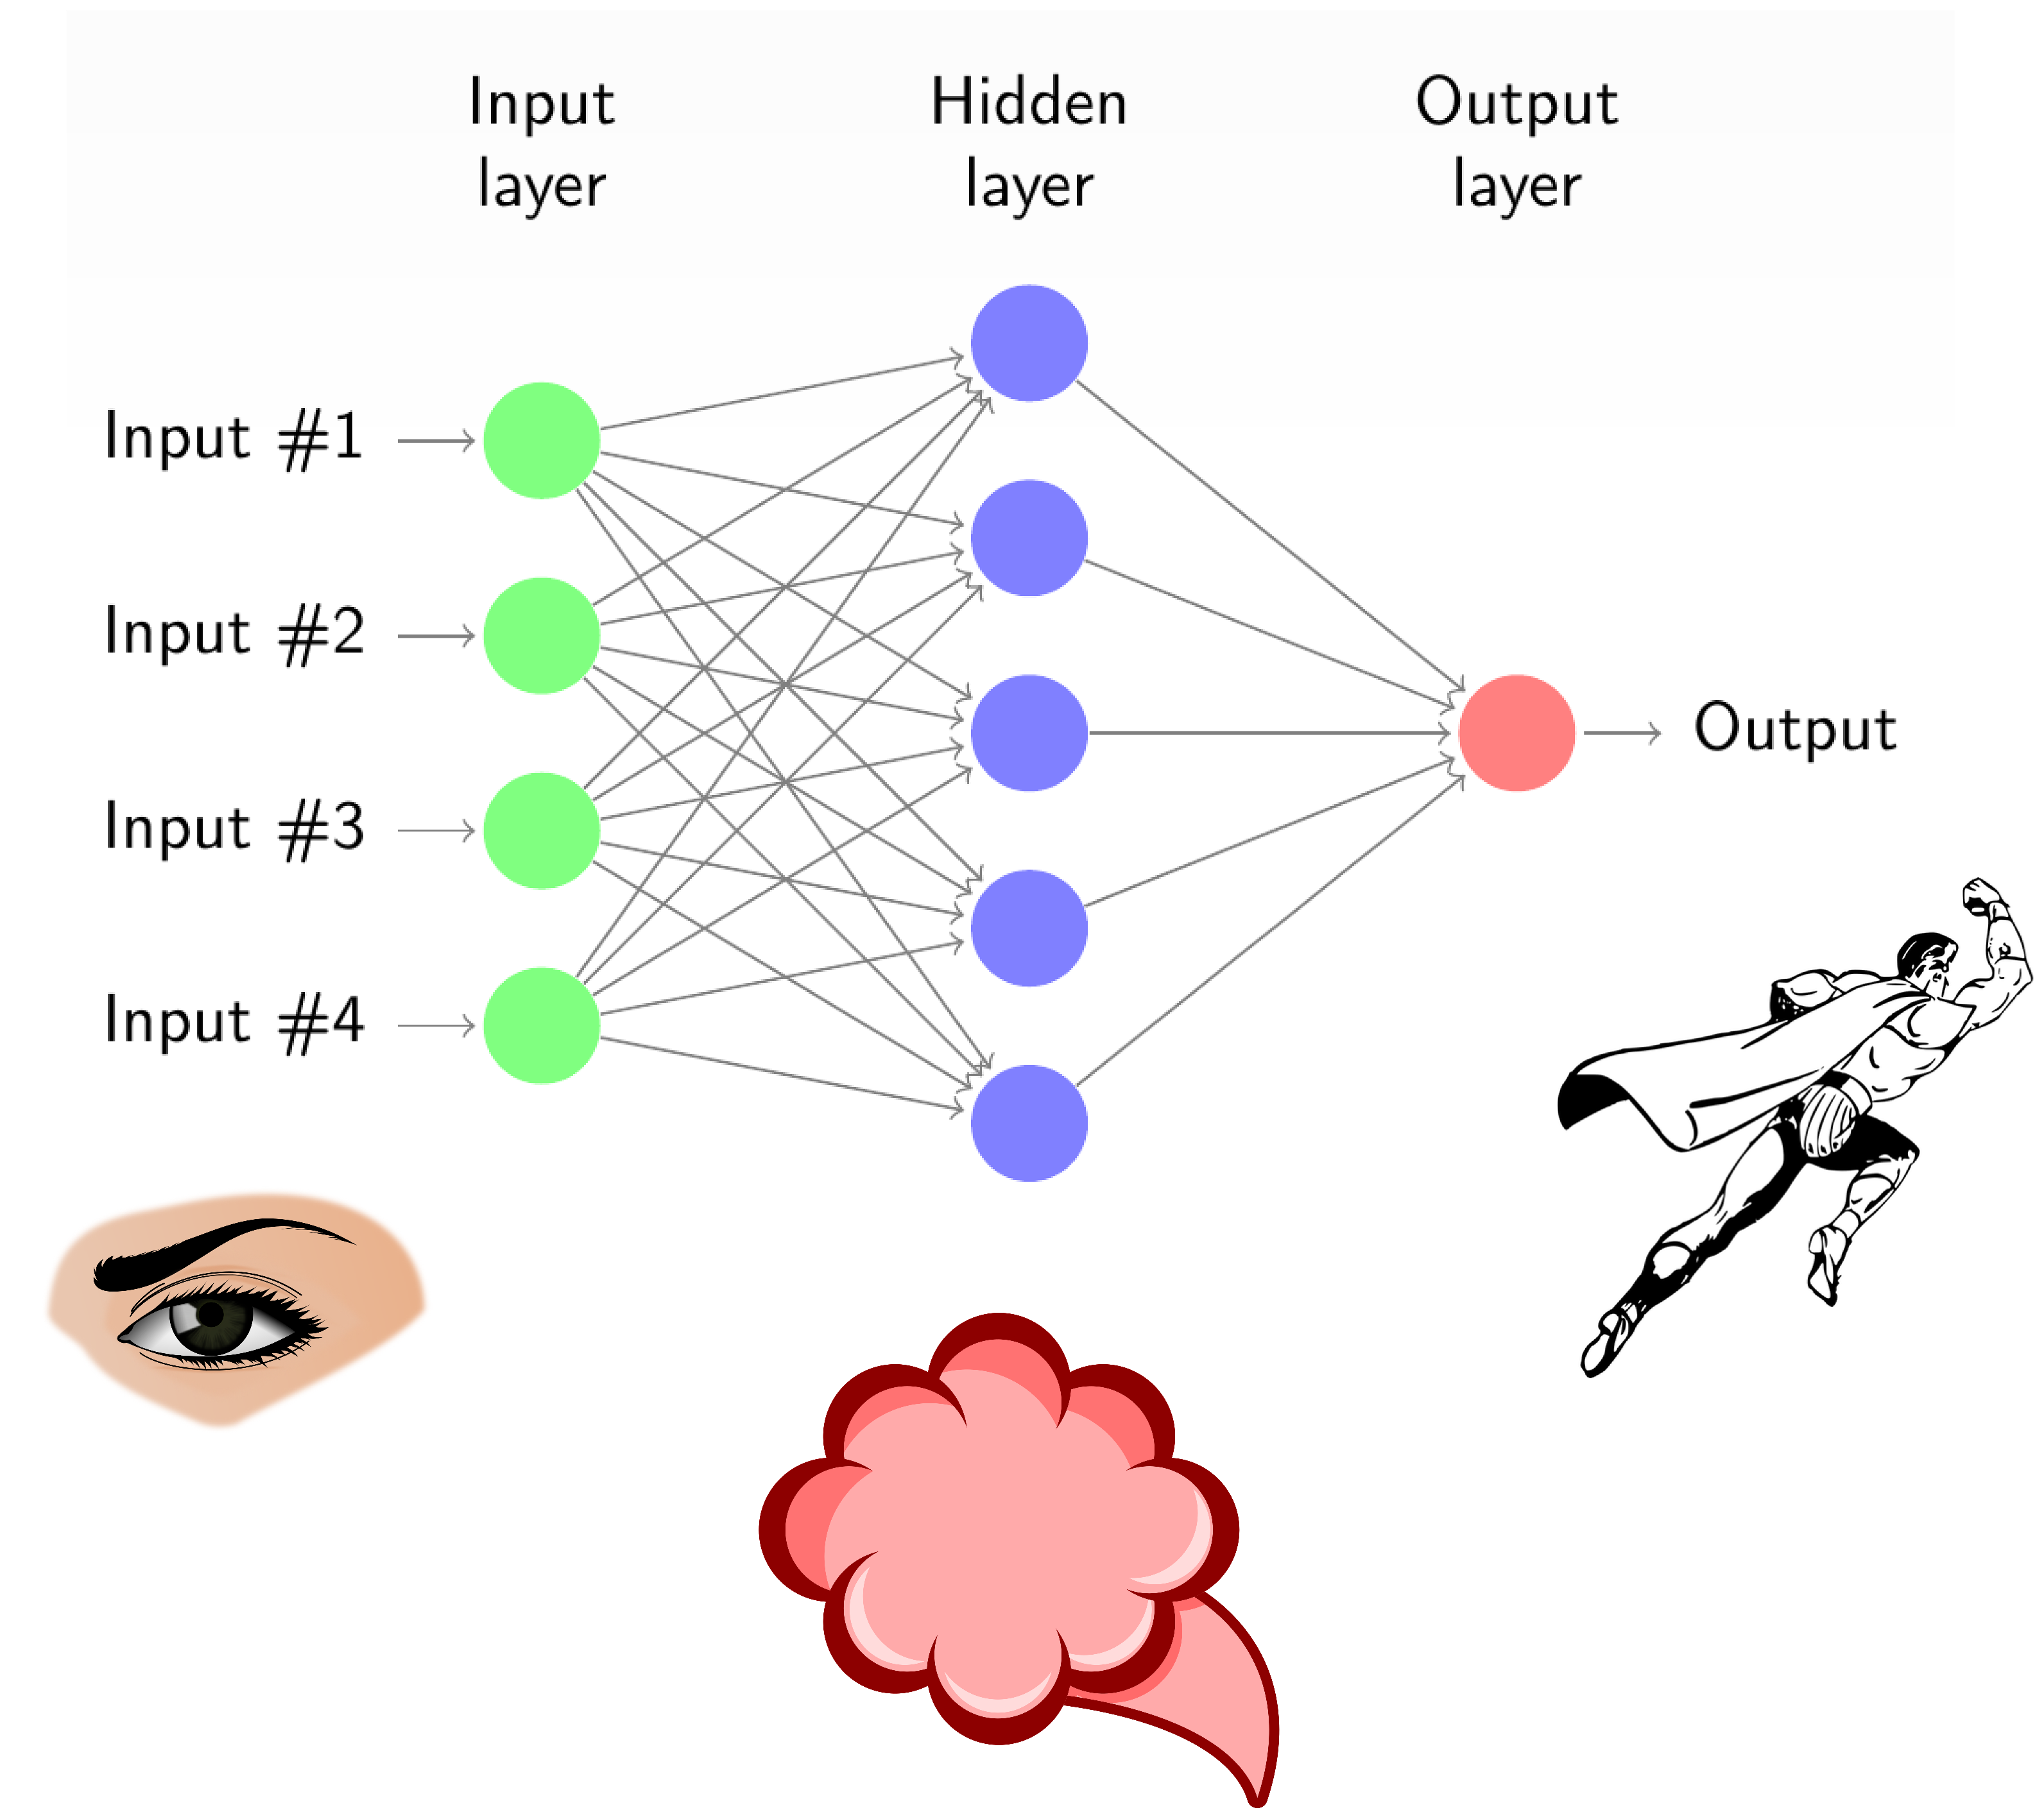
\includegraphics[width=0.8\textwidth]{net_structure}
\end{figure}
\end{frame}

\begin{frame}{Neural Networks - Choosing the next step}
\begin{tabular}{p{5cm}|p{5cm}}
    \begin{figure}
    	
\includegraphics[scale = 0.09]{brain}
    \end{figure}
    & 
    \begin{figure}
    	
\includegraphics[scale = 1.4]{machine}
    \end{figure} \\
  \multicolumn{1}{c|}{Evaluation of an action} & \multicolumn{1}{c}{Loss function} \\
    \begin{itemize}
        \item Simple perceptions: pain, satisfaction
        \item Expectation
    \end{itemize}
    & 
    \begin{itemize}
      \item Supervised learning: compare to the desired outcome
      \item Loss = estimator for quality
    \end{itemize} \\
\multicolumn{1}{c|}{Decision for a next step} & \multicolumn{1}{c}{Optimisation} \\
    \begin{itemize}
        \item Trial and error
        \item Learning from experience
    \end{itemize}
    & 
    \begin{itemize}
      \item Back-propagation impact of parameters' on the loss
      \item Adjust parameters to minimise plot
    \end{itemize} 
 \end{tabular}
\end{frame}

\begin{frame}{Hyperparameter optimisation}
    \begin{block}{What is a hyperparameter?}
        \begin{itemize}
            \item During the learning process the neural network optimises its internal parameters
            \item Some parameters are still set by the user according to the task of the network
            \item These are called hyperparameters
        \end{itemize}
        
    \end{block}
    \begin{block}{How does one optimise the choice?}
        \begin{itemize}
            \item Neural networks provide several metrics to estimate result and performance
            \item To optimise the hyperparameters one usually runs several configurations to find a good set of parameters
        \end{itemize}
    \end{block}
\end{frame}


\begin{frame}{Concepts of evolutionary network optimisation}
    \begin{block}{Choosing a start}
        \begin{itemize}
            \item Randomly choose a set of values for each hyperparameter
            \item Combine the random selection to create a set of network configurations
        \end{itemize}
    \end{block}
    \begin{block}{Evaluating a start}
        \begin{itemize}
            \item Run the networks for a small number of epochs
            \item Use networks' metrics to evaluate the performance
        \end{itemize}
    \end{block}
    \begin{block}{Choosing a next step}
        \begin{itemize}
            \item Rank networks by their metrics
            \item Reuse, mate and mutate networks
        \end{itemize}
    \end{block}
\end{frame}

\begin{frame}{The initial generation}
    \begin{block}{Current setup}
        \begin{itemize}
            \item Choose a random set of hyperparameters from a range of paramters set by the user
            \item Create a set of neural networks from all possible combinations
        \end{itemize}
    \end{block}
    \begin{block}{Planned}
        \begin{itemize}
            \item Draw each hyperparameter from a fitting distribution
            \item Restrict the number of combinations based on the hyperparameter
        \end{itemize}
    \end{block}
\end{frame}

\begin{frame}{Evaluating a generation}
    \begin{block}{Current setup}
        \begin{itemize}
            \item Evaluate all networks based on a metric of choice
            \item The metric of choice can be simply the AUC
            \item Save the $x$ best configuration
        \end{itemize}
    \end{block}
    \begin{block}{Planned}
        \begin{itemize}
            \item Test and combine different metrics
            \item Implement different metrics with regard to early stopping
        \end{itemize}
    \end{block}
\end{frame}

\begin{frame}{Breeding the next generation}
    \begin{block}{Current setup}
        \begin{itemize}
            \item Always keep the best configuration
            \item Recombine the $\lambda$ best configurations
            \item Recombine the $\lambda$ best generations again and vary $\mu$ hyperparameters
        \end{itemize}
    \end{block}
    \begin{block}{Planned}
        \begin{itemize}
            \item Include more hyperparameters
            \item Specify different variation probabilities and values for different hyperparameters
        \end{itemize}
    \end{block}
\end{frame}

\begin{frame}{Summary of the optimisation process}
    \begin{columns}
    \begin{column}{0.5\textwidth}
        \begin{itemize}
            \item Survival of the fittest: Keep the best setup
            \item Recombination: Reuse the best hyperparameters for the next batch
            \item Variation: Randomly change the hyperparamters to avoid local minima and bias
        \end{itemize}
    \end{column}
    \begin{column}{0.5\textwidth}
        \begin{figure}
            \centering
            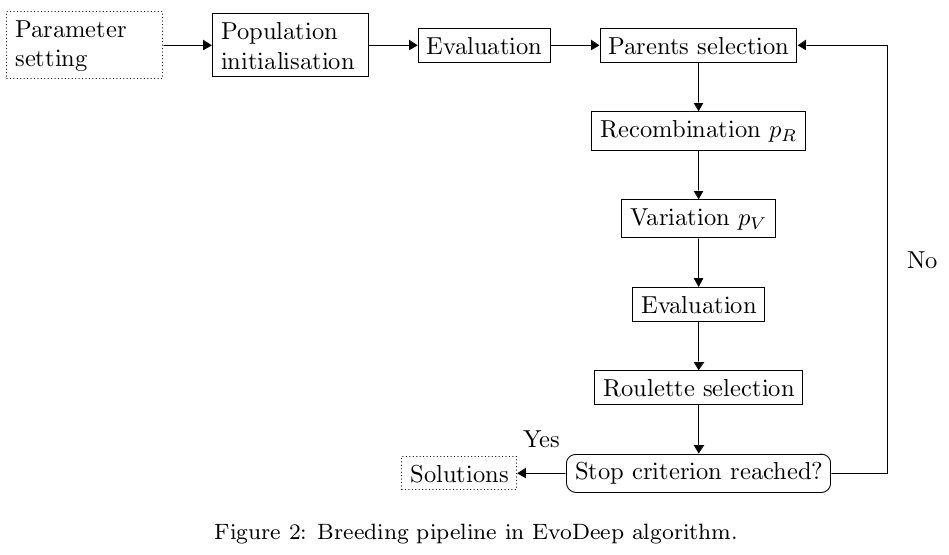
\includegraphics[width=\textwidth]{breed.png}
            \caption{\cite{naranjo}}
        \end{figure}
    \end{column}
    \end{columns}
\end{frame}
\section{\tHq}
\begin{frame}
    \begin{center}
        \Huge \tHq \\ A binary classifier
    \end{center}
\end{frame}

\begin{frame}{Hyperparameters}
  \begin{itemize}
    \item Optimised by small grid search
  \end{itemize}
    \begin{table}[]
    \begin{tabular}{|l|l|}
    \hline
    Hyperparameter          &     Setting              \\ \hline
    Model                   &     Binary          \\ \hline
    Nodes                   &     120                  \\ \hline
    Layers                  &     6                    \\ \hline
    Dropout                 &     0.65                 \\ \hline
    Batchnormalisation      &     On                   \\ \hline
    Activation              &     elu                  \\ \hline
    Output activation       &     sigmoid              \\ \hline
    Batch size              &     1000                 \\ \hline
    Optimisation            &     Adam                 \\ \hline
    Weight Initialisation   &     Lecun Normalisation  \\ \hline
    K-folds                 &     4                    \\ \hline
    \end{tabular}
    \end{table}
\end{frame}

\begin{frame}{Results}
    \begin{columns}
        \begin{column}{0.5\textwidth}
          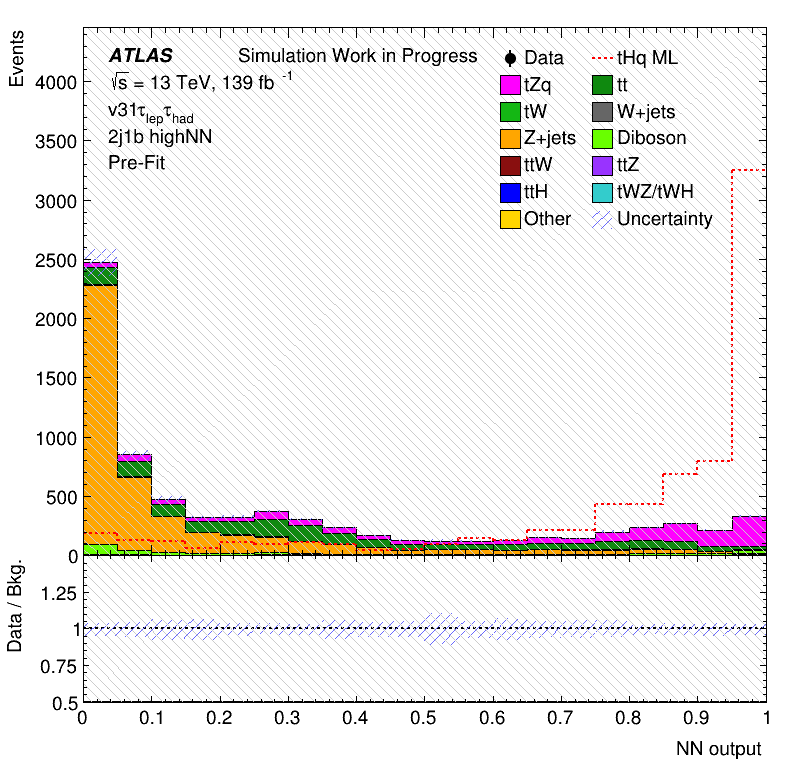
\includegraphics[width=0.82\textwidth]{response_binary}
          \begin{itemize}
            \item Decent separation
            \item Stable agreement
          \end{itemize}
        \end{column}
        \begin{column}{0.5\textwidth}
          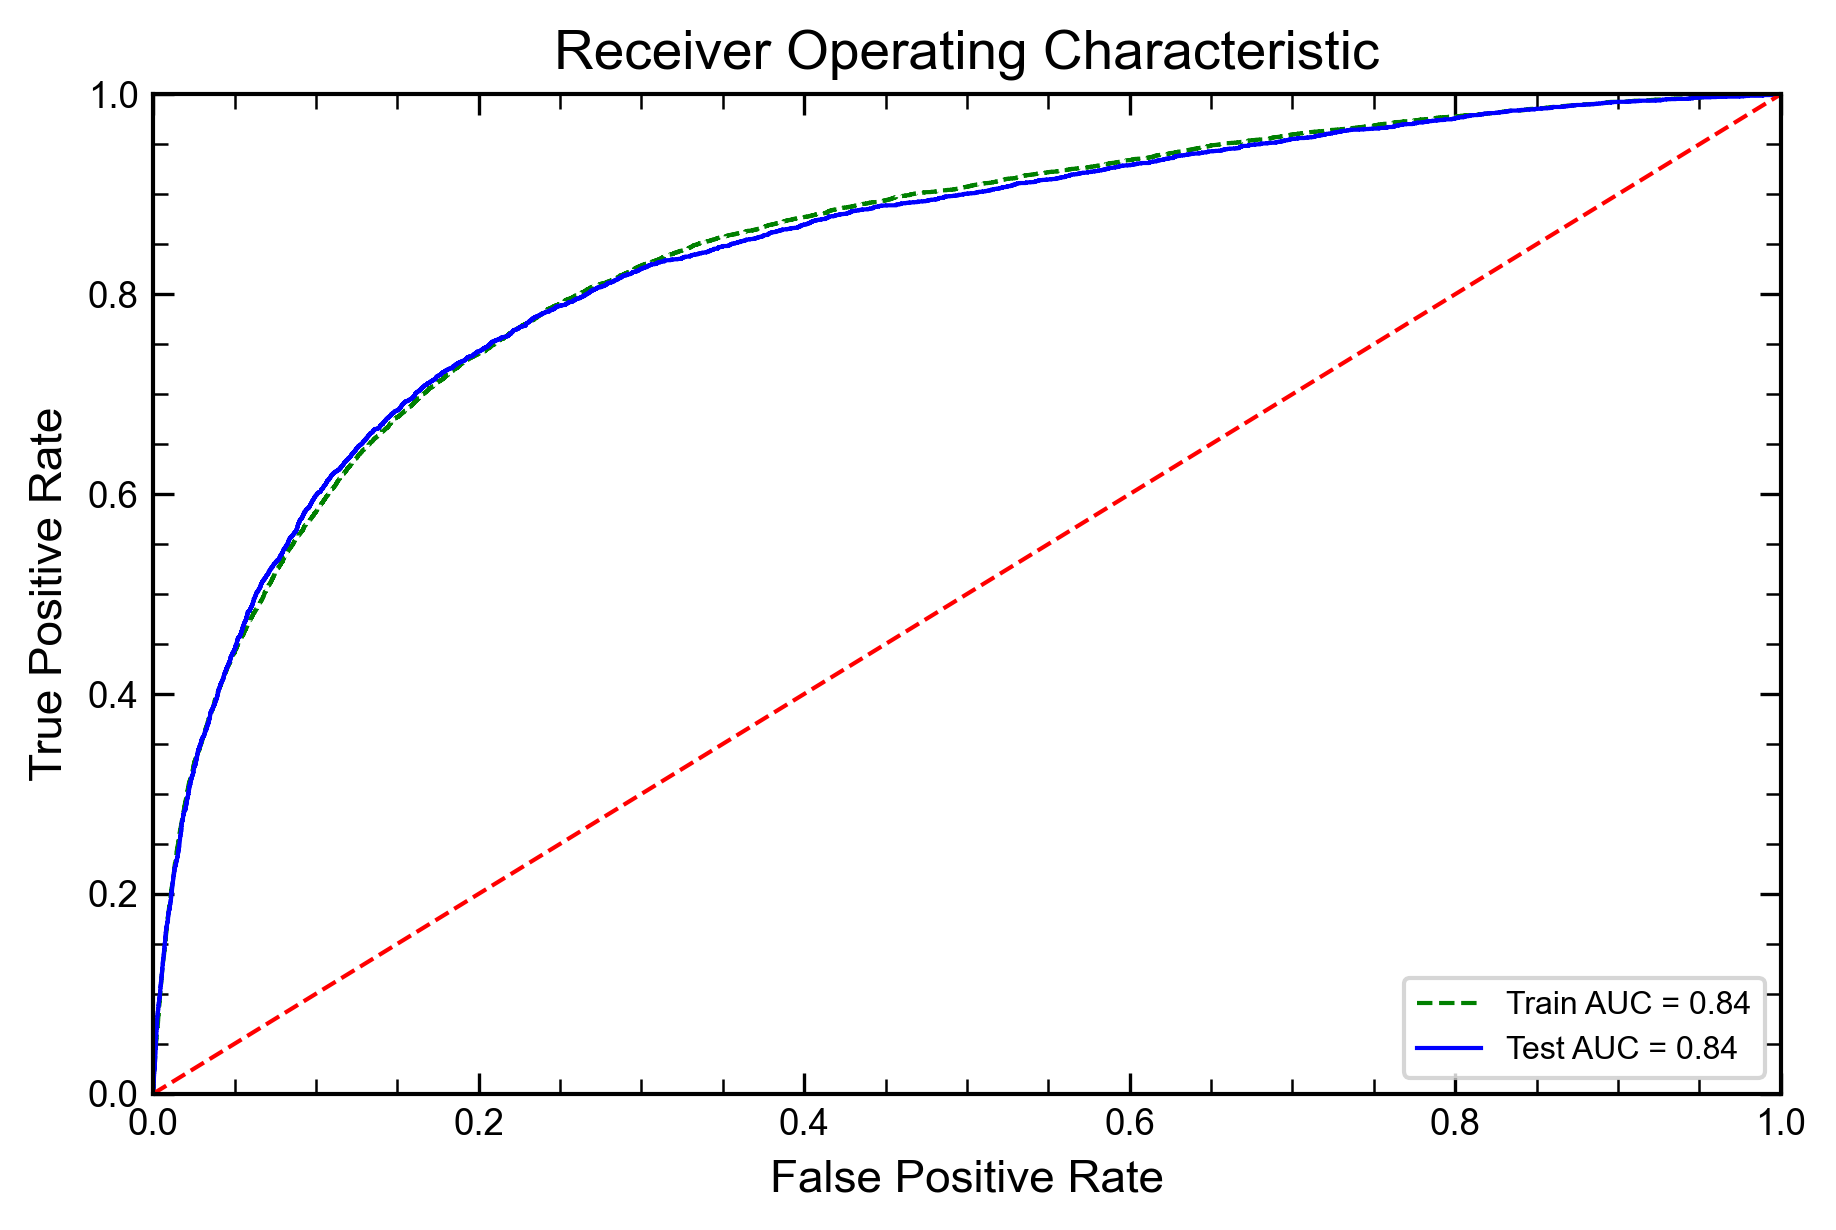
\includegraphics[width=0.84\textwidth]{ROC_binary}
          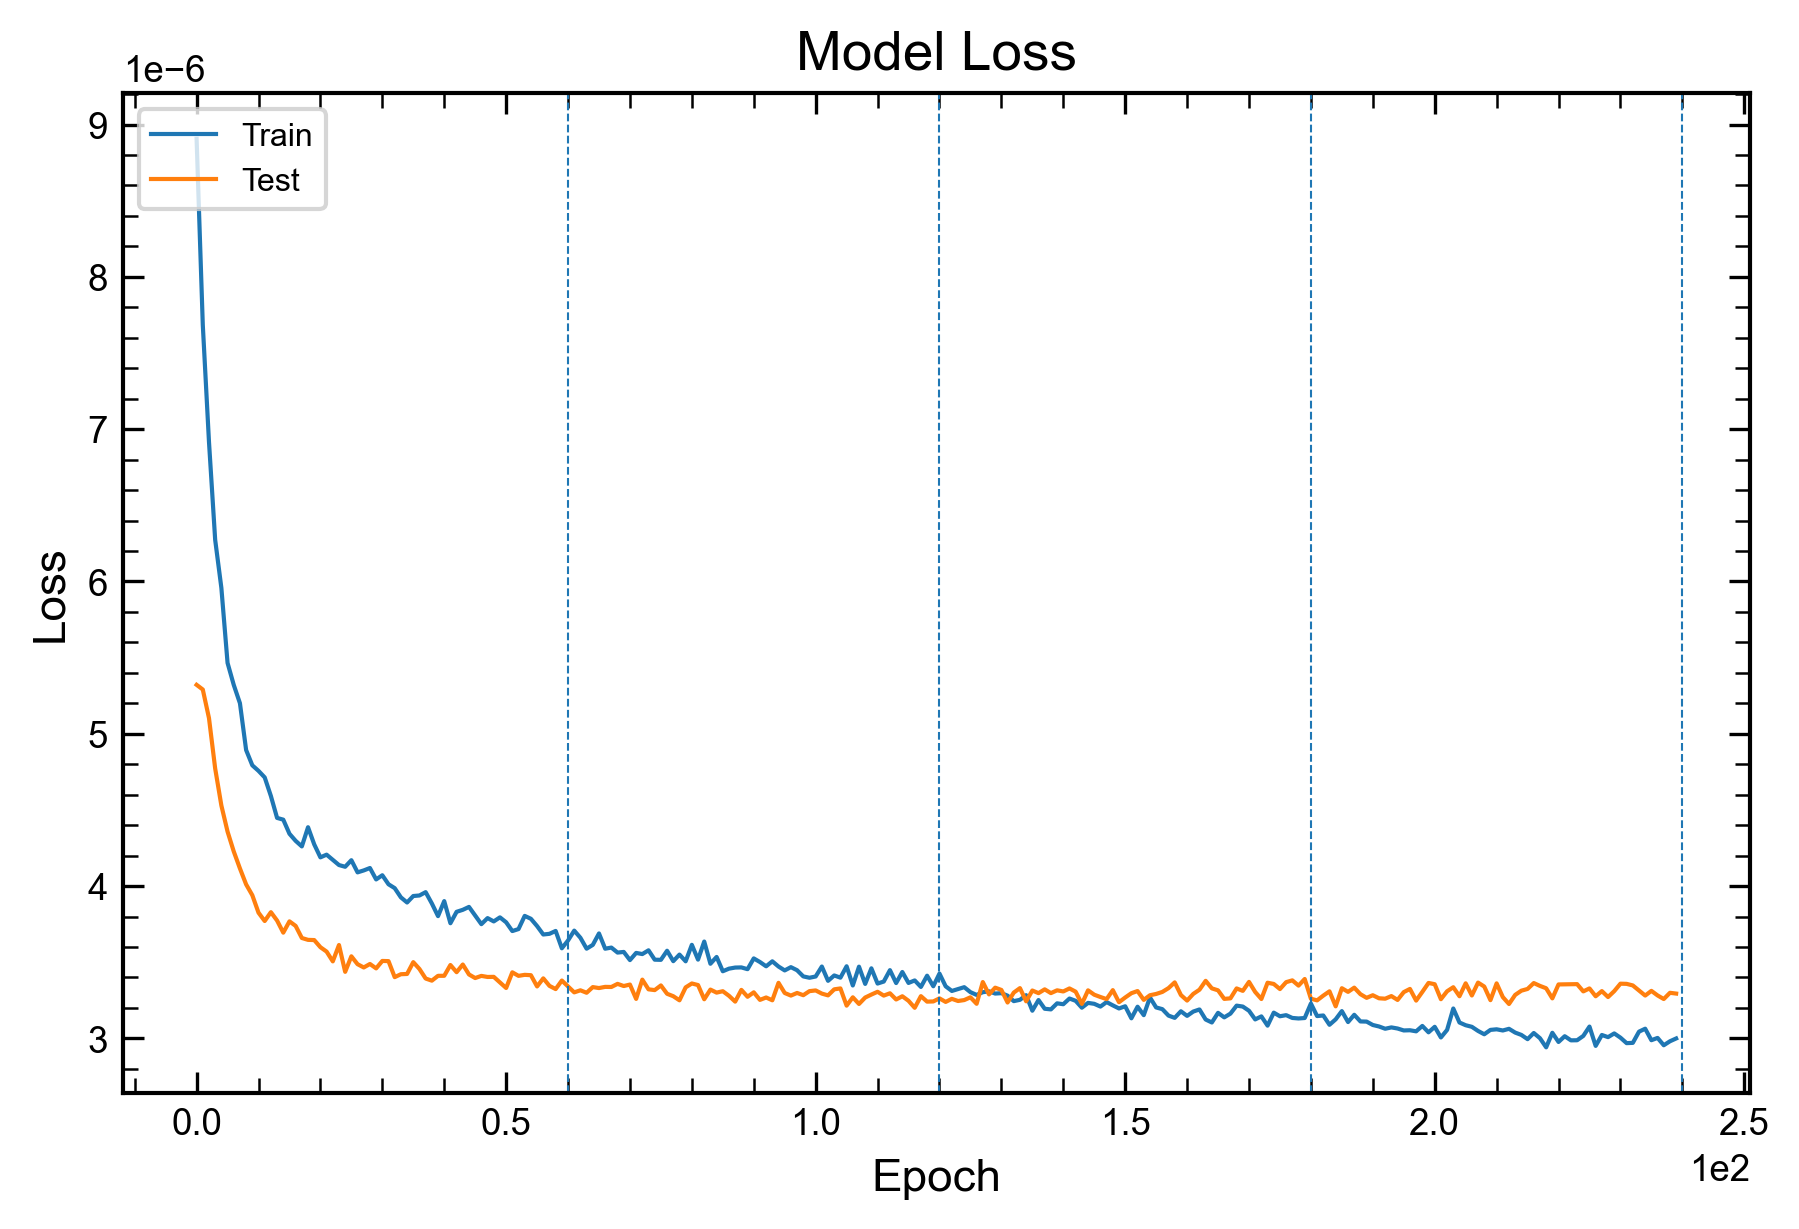
\includegraphics[width=0.84\textwidth]{loss_binary}
        \end{column}
    \end{columns}    
\end{frame}

\begin{frame}
    \begin{center}
        \Huge \tHq \\ A closer look
    \end{center}
\end{frame}

\begin{frame}{The ROC curve}
  \centering 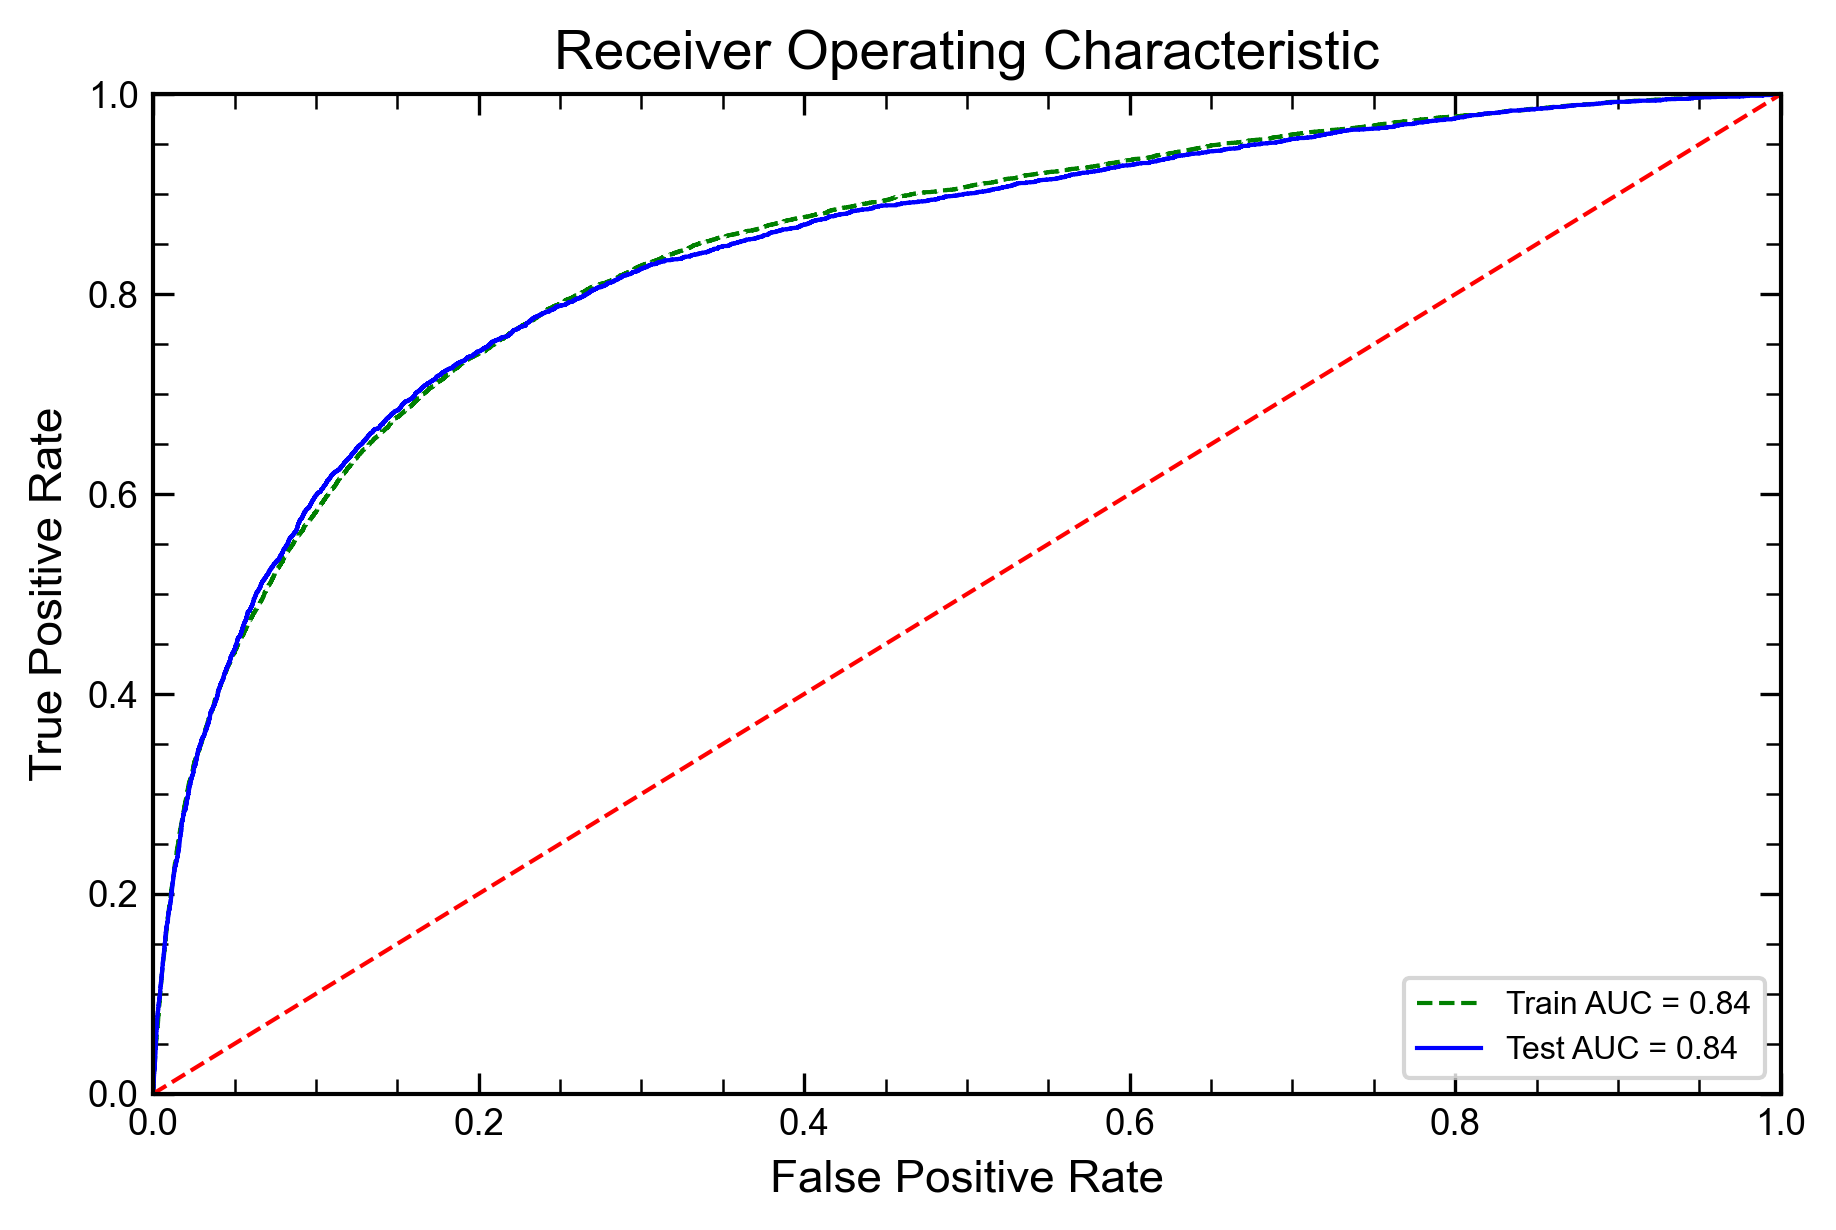
\includegraphics[width=0.8\textwidth]{ROC_binary}
  \begin{itemize}
    \item AUC = Are Under the Curve
    \item Good estimator for model quality
  \end{itemize}
\end{frame}

\begin{frame}{The loss curve}
  \centering 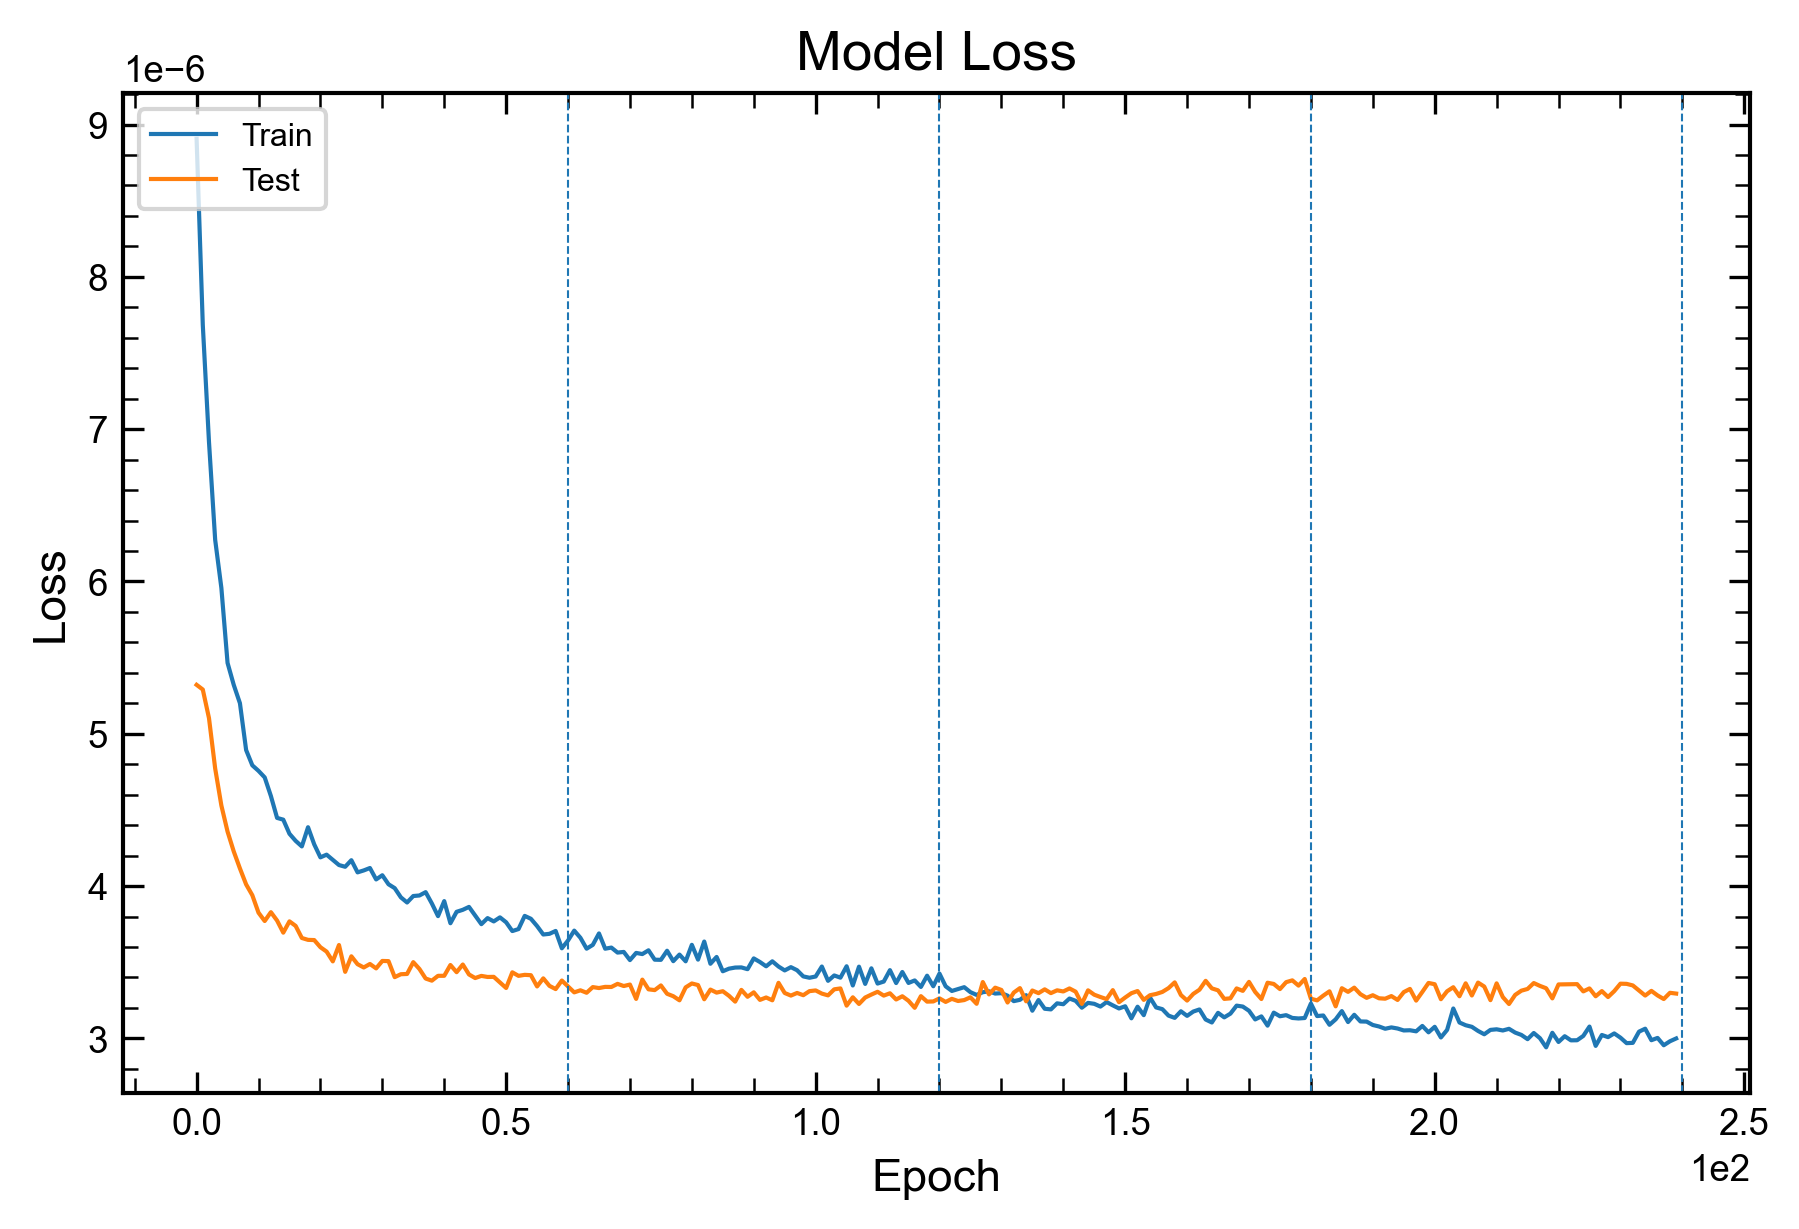
\includegraphics[width=0.8\textwidth]{loss_binary}
\begin{itemize}
  \item Should decrease
  \item Should not diverge
\end{itemize}
\end{frame}

\begin{frame}{The response}
  \centering 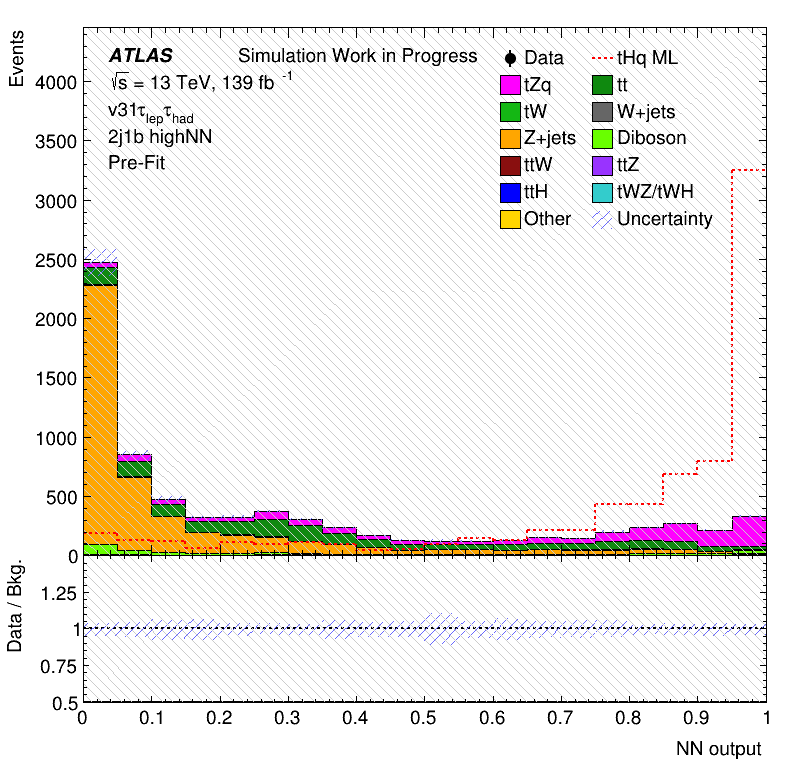
\includegraphics[width=0.6\textwidth]{response_binary}
  \begin{itemize}
    \item Seeing a separation is good
    \item Signal should be right
  \end{itemize}
\end{frame}

\begin{frame}
    \begin{center}
        \Huge \tZq \\ Weakness in a binary separation
    \end{center}
\end{frame}

\begin{frame}{Response}
    \centering 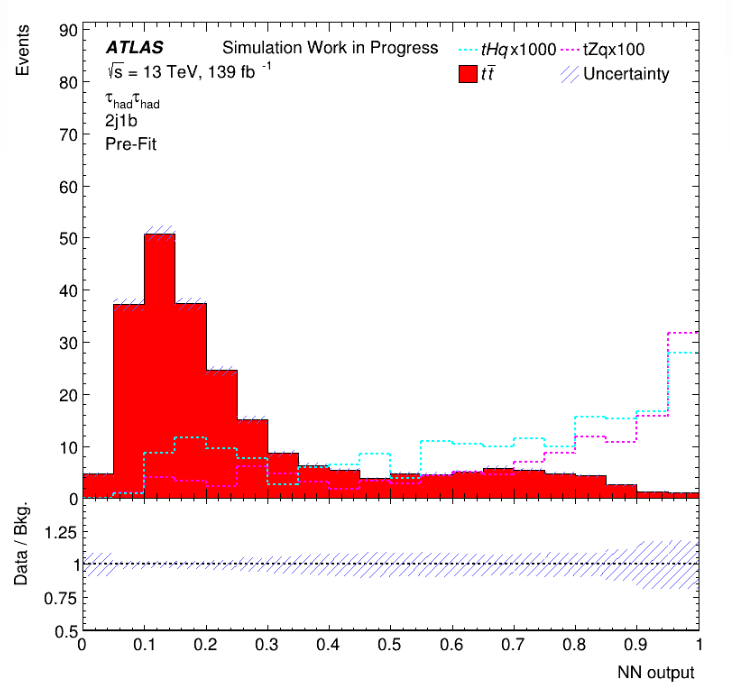
\includegraphics[width=0.81\textwidth]{tZq_problem}
\end{frame}
\section{Categorical}
\begin{frame}
    \begin{center}
        \Huge Categorical Neural Networks
    \end{center}
\end{frame}

\begin{frame}{The idea of categorical neural networks}
    \begin{itemize}
        \item \Large Difficult backgrounds $\rightarrow$ additional targets
    \end{itemize}
\end{frame}

\begin{frame}{Target handling}
    \begin{itemize}
        \item Using One-Hot-Encoding
        \vspace{0.23cm}
        \item Vector instead of target
        \vspace{0.23cm}
        \item Target values get translated to vector component
    \end{itemize}
    \vspace{0.23cm}
    \begin{equation*}
    \tHq = \begin{bmatrix}
           0 \\
           0 \\
           1
         \end{bmatrix}
    \tZq = \begin{bmatrix}
           1 \\
           0 \\
           0
         \end{bmatrix}
    Background = \begin{bmatrix}
           0 \\
           1 \\
           0
         \end{bmatrix}
    \end{equation*}
\end{frame}

\begin{frame}{Binary final node - Sigmoid}
    \begin{columns}
        \begin{column}{0.65\textwidth}
            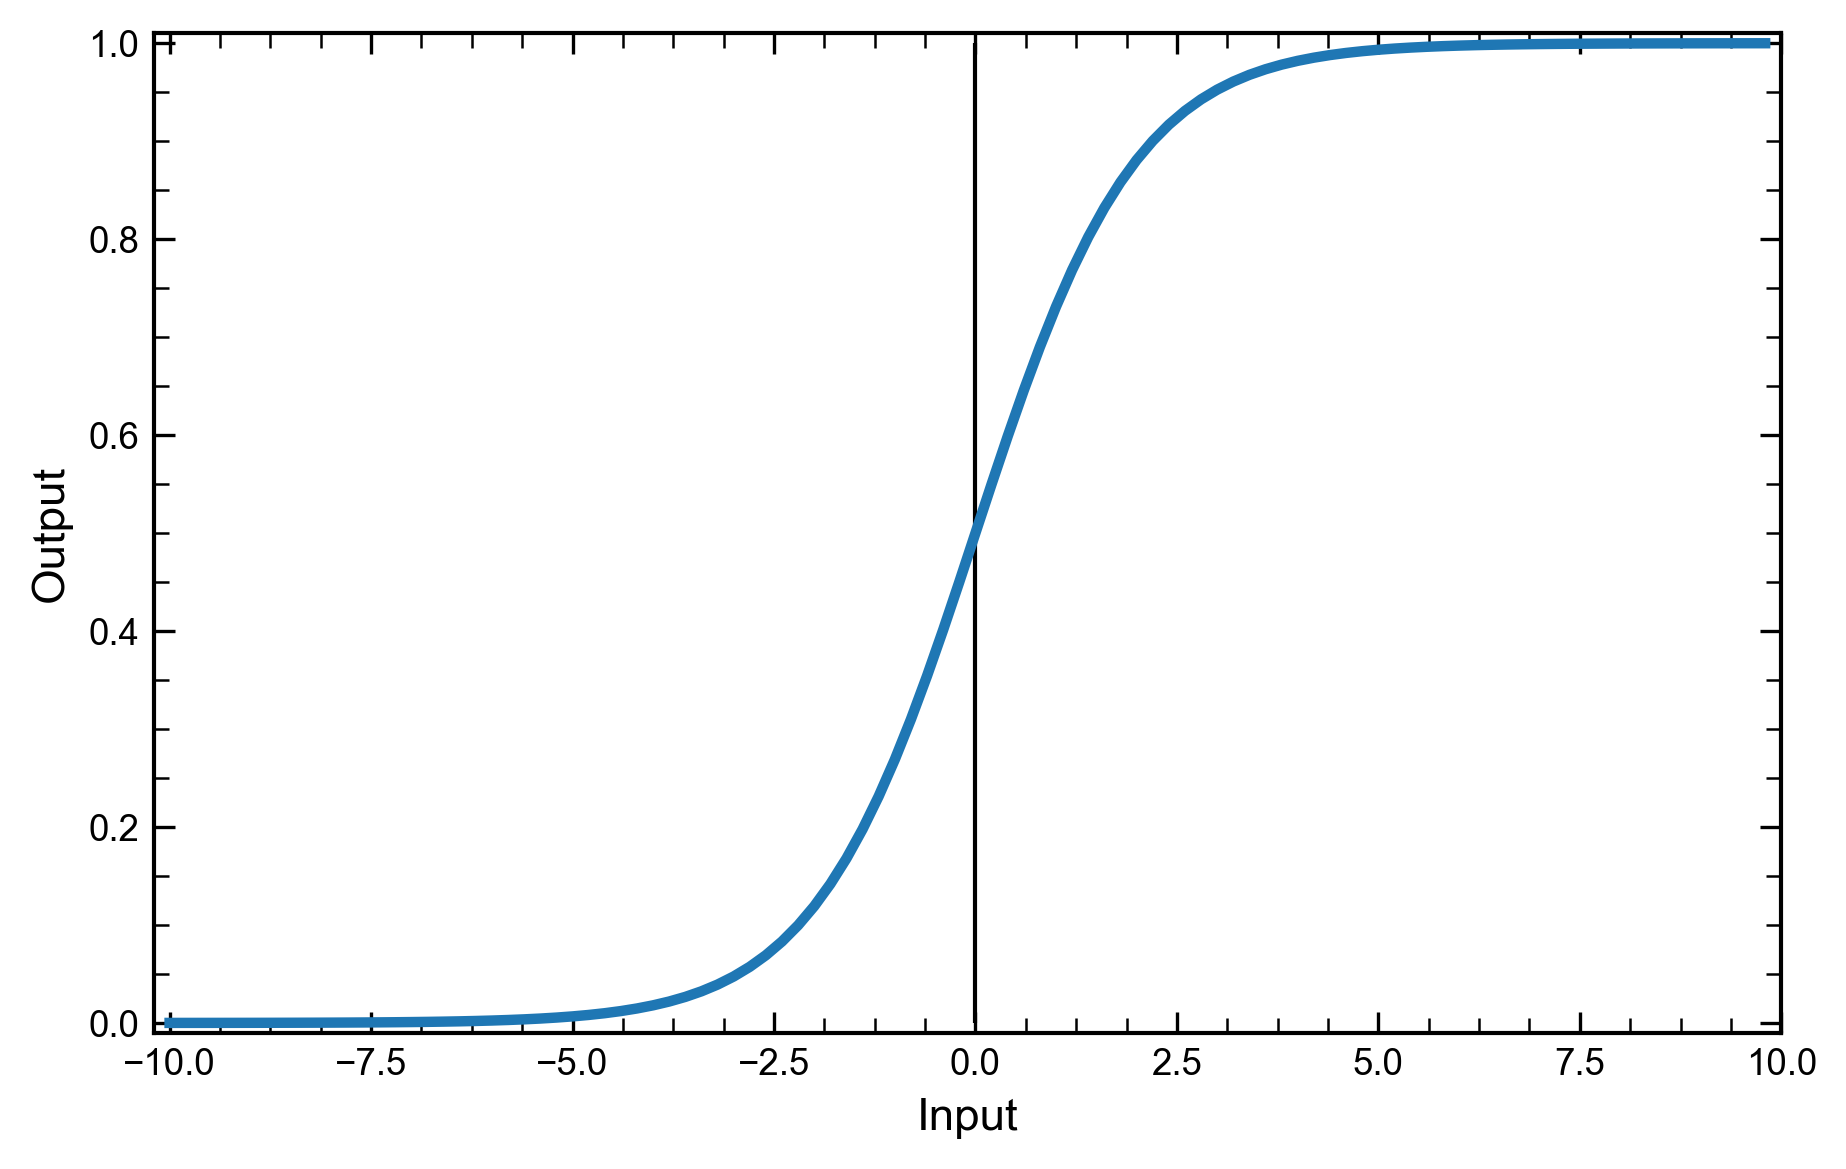
\includegraphics[width=\textwidth]{sigmoid}
        \end{column}
        \begin{column}{0.5\textwidth}
            \begin{itemize}
                \item Bounded, differentiable
                \item Allows for backpropagation
                \item Assigning a single output value $\in (0,1)$
            \end{itemize}
            \begingroup
            \large
            \begin{equation*}
                \frac{1}{1+e^{-s_i}}
            \end{equation*}
            \endgroup
        \end{column}
    \end{columns}
    \begin{itemize}
        \color{red}
        \item Expects only one input value
    \end{itemize}
\end{frame}

\begin{frame}{Categorical final node - Softmax}
    \begin{columns}
        \begin{column}{0.5\textwidth}
            \begingroup
            \huge
            \begin{equation*}
                f(s)=\frac{e^{s_i}}{\sum_j^c e^{s_j}}
            \end{equation*}
            \endgroup
        \end{column}
        \begin{column}{0.5\textwidth}
            \begin{itemize}
                \item Takes an input vector equal to the number of targets
                \vspace{0.1cm}
                \item Sum of vector components is 1
                \vspace{0.1cm}
                \item normalises output to a probability distribution
            \end{itemize}
        \end{column}
    \end{columns}
\end{frame}

\begin{frame}{Loss function - Crossentropy}
    \begin{columns}
        \begin{column}{0.5\textwidth}
            \begin{block}{Binary Crossentropy}
                \begin{equation*}
                    Loss = - \sum_{i=1} y_i \log \hat{y}_i =
                \end{equation*}
                \begin{equation*}
                    -y_1 \log \hat{y_1} - (1-y_1) \log (1-\hat{y}_1)
                \end{equation*}
                \begin{itemize}
                    \item Measures model quality for two classes
                \end{itemize}
            \end{block}
        \end{column}
        \begin{column}{0.5\textwidth}
            \begin{block}{Categorical Crossentropy}
                \begin{equation*}
                    Loss = - \sum_{i=1} y_i \log \hat{y_i}
                \end{equation*}
                \begin{itemize}
                    \item Measures model quality for multiple classes
                \end{itemize}
            \end{block}
        \end{column}
    \end{columns}
\end{frame}

\begin{frame}{Hyperparameters}
    \begin{table}[]
    \begin{tabular}{|l|l|}
    \hline
    Hyperparameter          &     Setting              \\ \hline
    Model                   &     Categorical          \\ \hline
    Nodes                   &     120                  \\ \hline
    Layers                  &     6                    \\ \hline
    Dropout                 &     0.65                 \\ \hline
    Batchnormalisation      &     On                   \\ \hline
    Activation              &     elu                  \\ \hline
    Output activation       &     Softmax              \\ \hline
    Batch size              &     1000                 \\ \hline
    Optimisation            &     Adam                 \\ \hline
    Weight Initialisation   &     Lecun Normalisation  \\ \hline
    K-folds                 &     4                    \\ \hline
    \end{tabular}
    \end{table}
\end{frame}

\begin{frame}{Results}
    \begin{columns}
        \begin{column}{0.5\textwidth}
          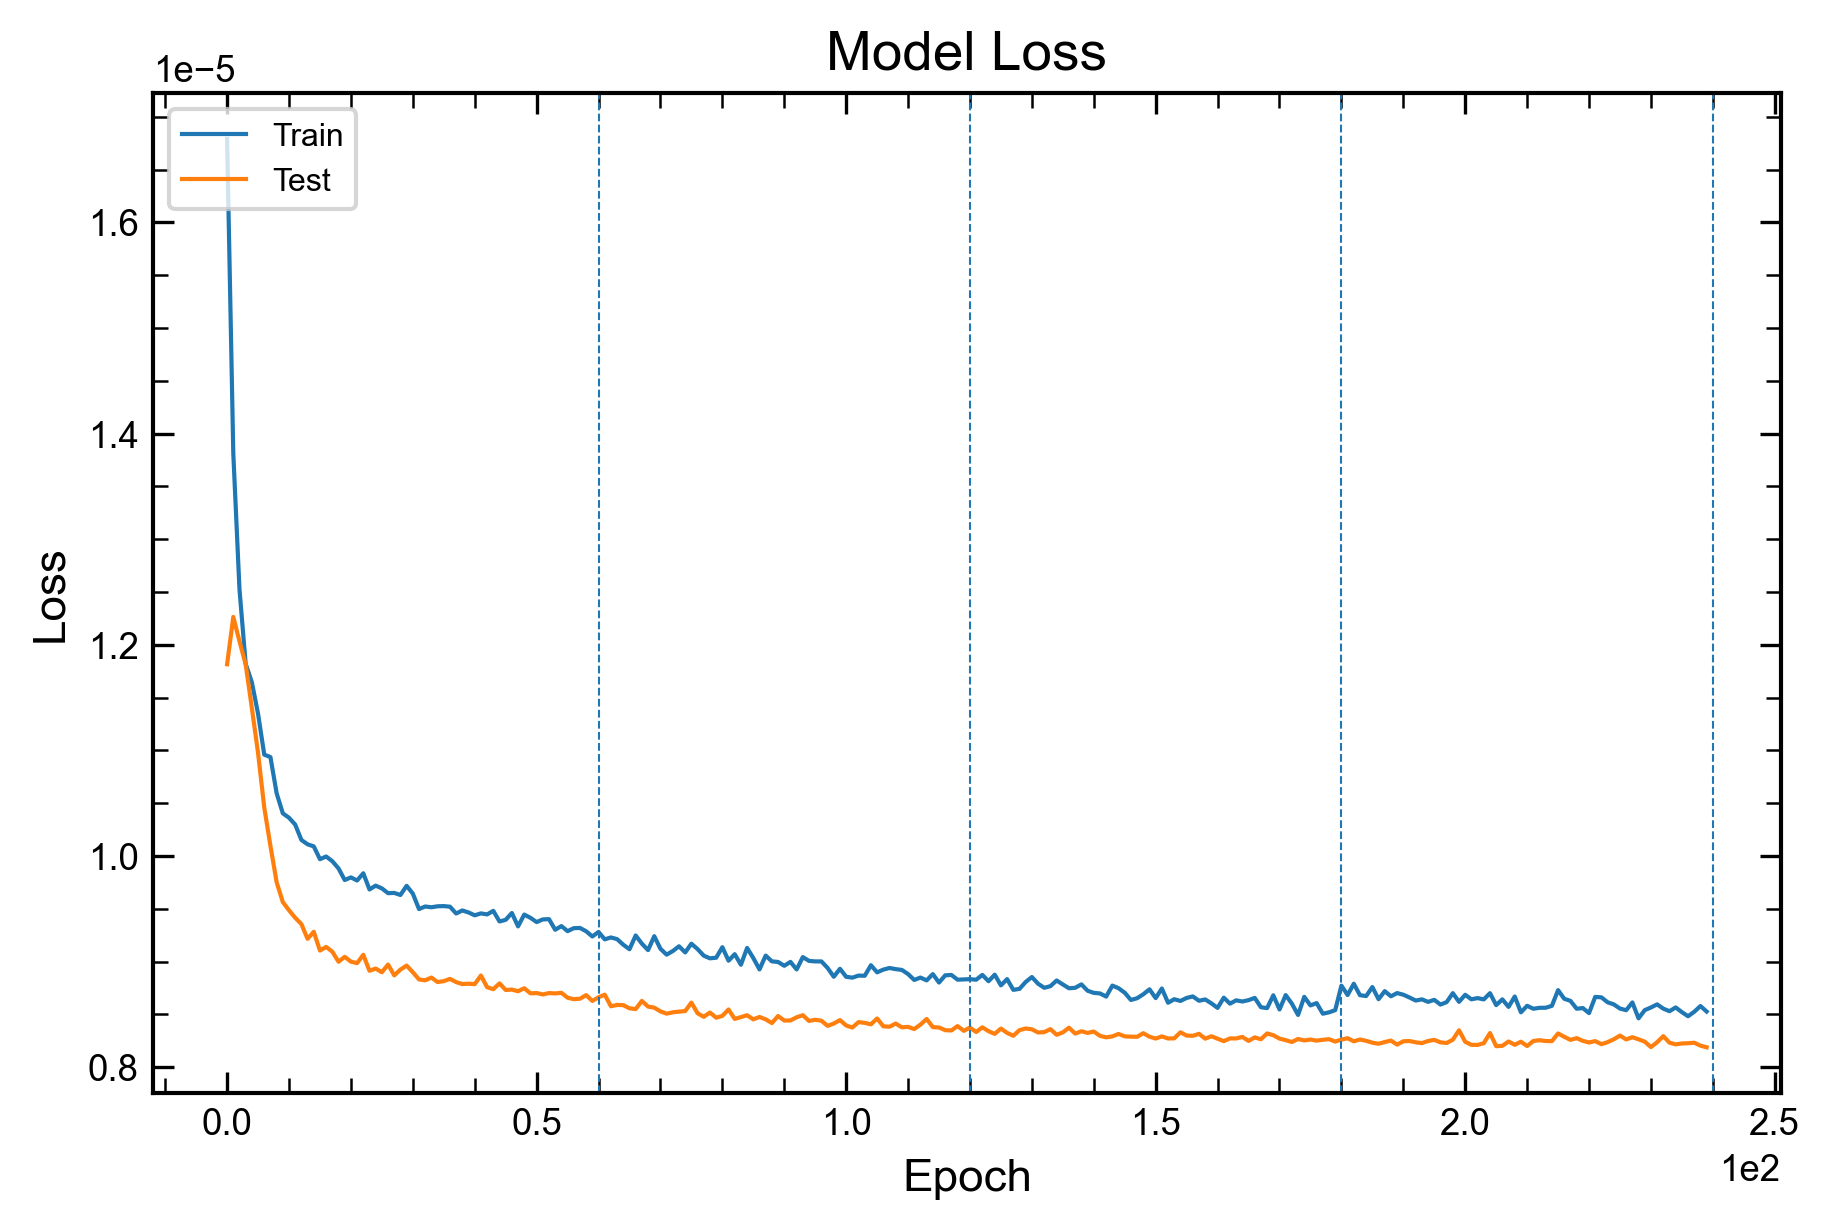
\includegraphics[width=0.8\textwidth]{losses_cat}
          \begin{itemize}
            \item Stable training
            \item Good AUC
          \end{itemize}
        \end{column}
        \begin{column}{0.5\textwidth}
          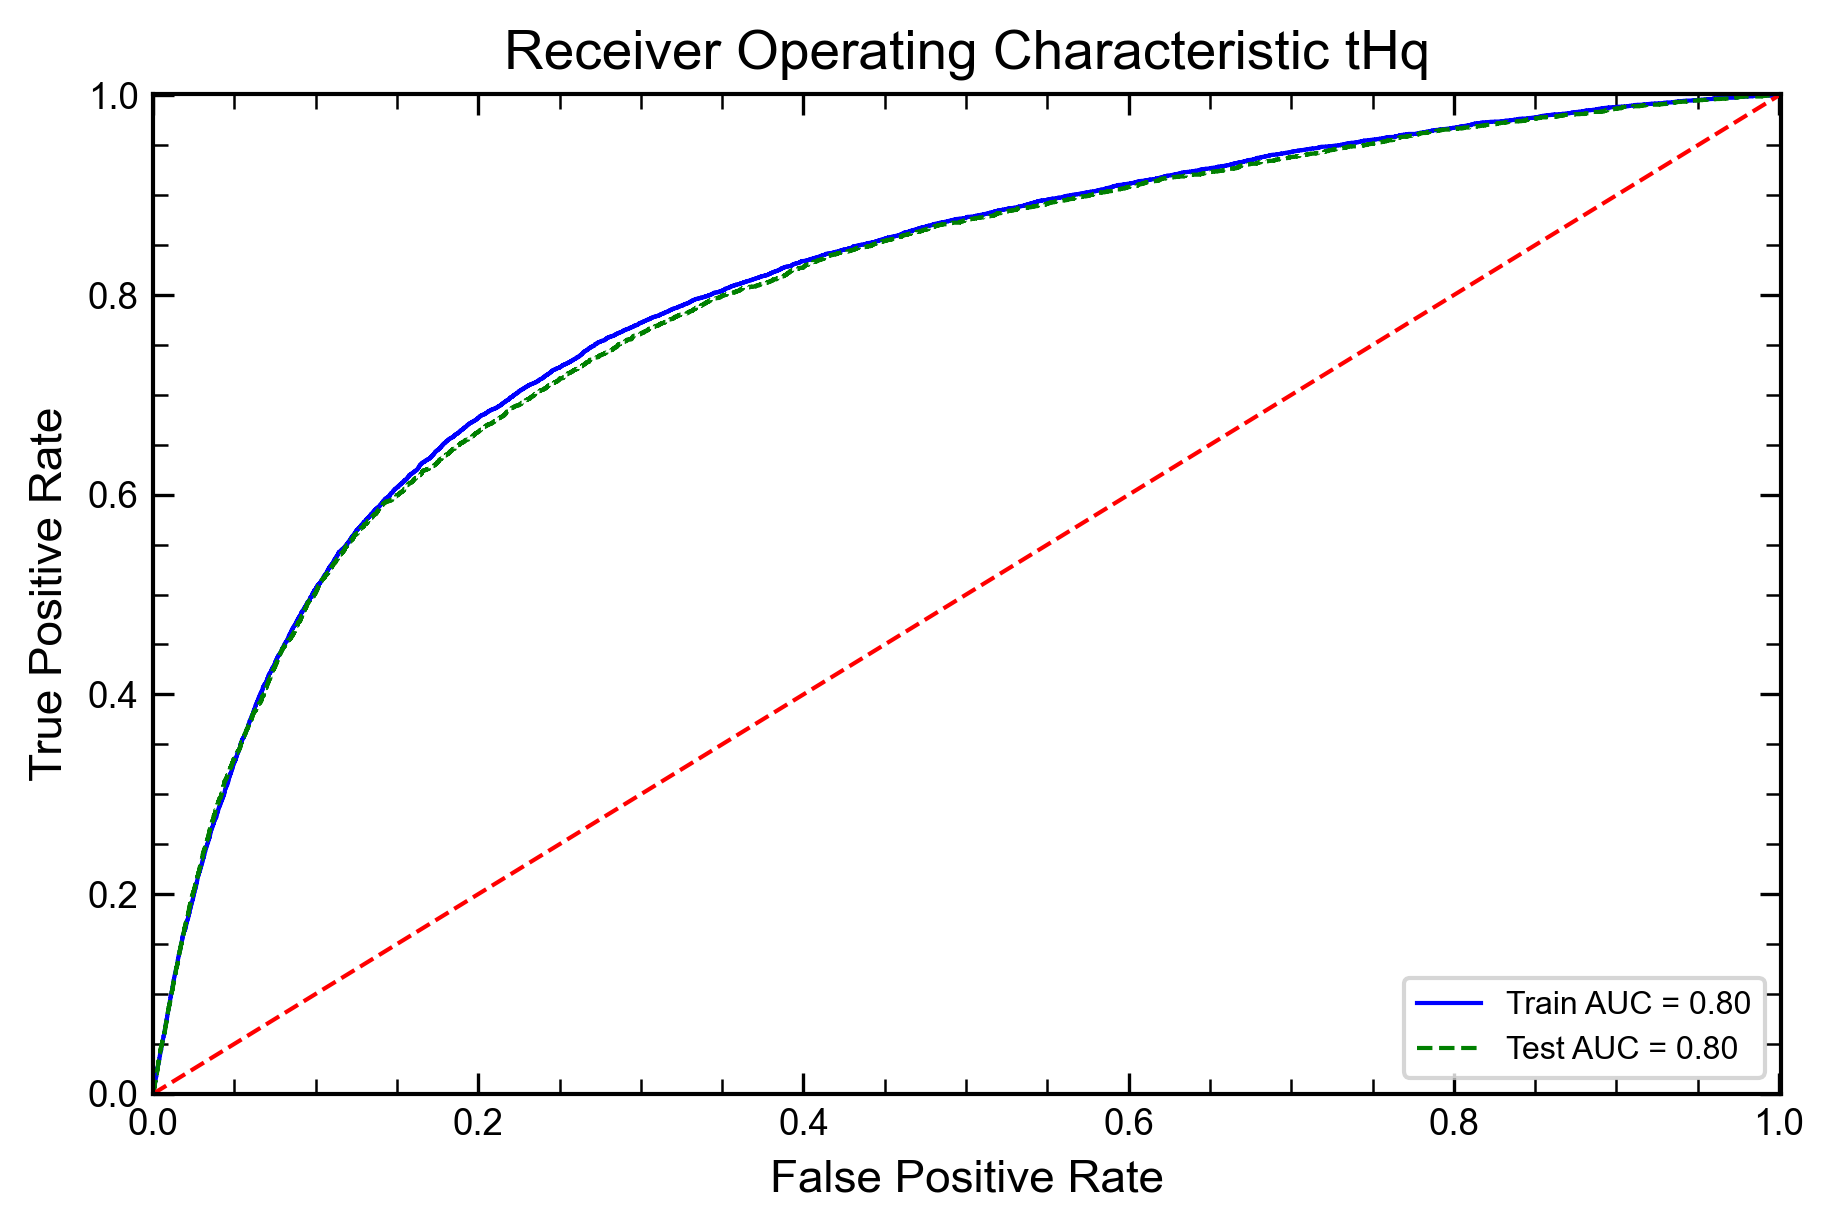
\includegraphics[width=0.8\textwidth]{ROC_cat}
          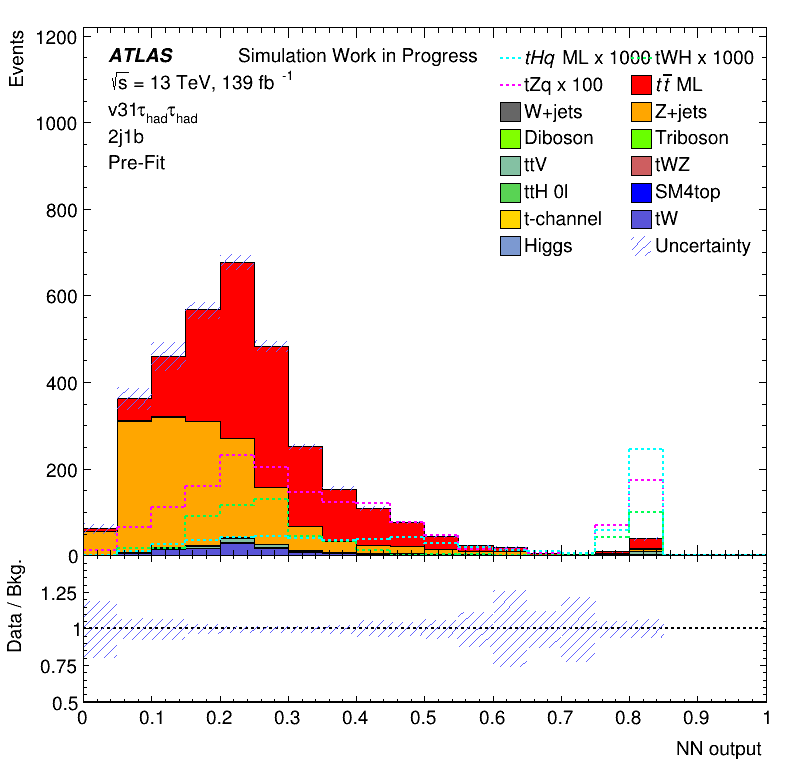
\includegraphics[width=0.8\textwidth]{response_cat}
        \end{column}
    \end{columns}    
\end{frame}

\begin{frame}{Response}
      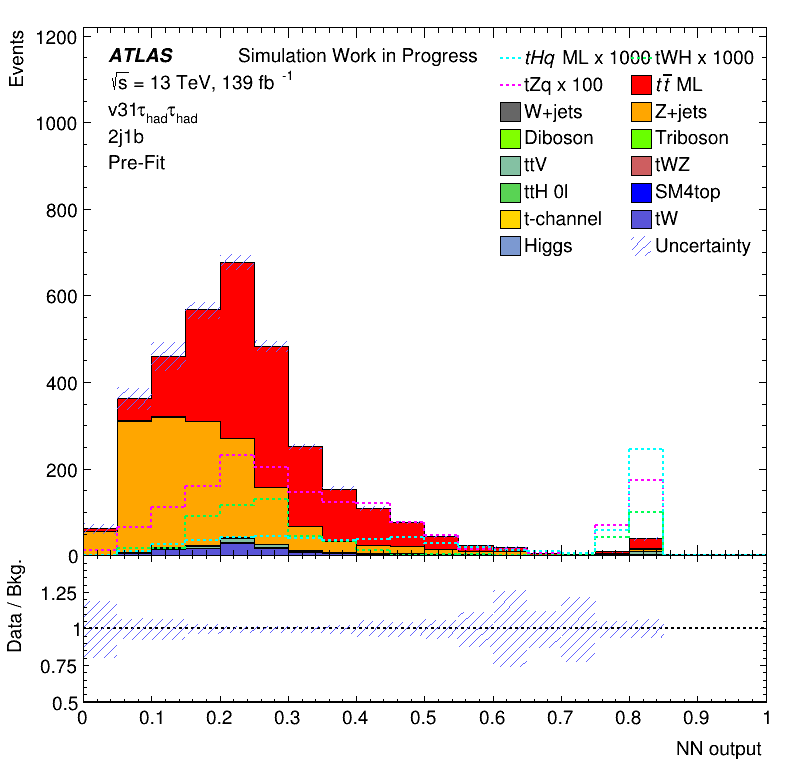
\includegraphics[width=0.75\textwidth]{response_cat}
\end{frame}

\begin{frame}{Additional responses}
  \begin{columns}
    \begin{column}{0.5\textwidth}
      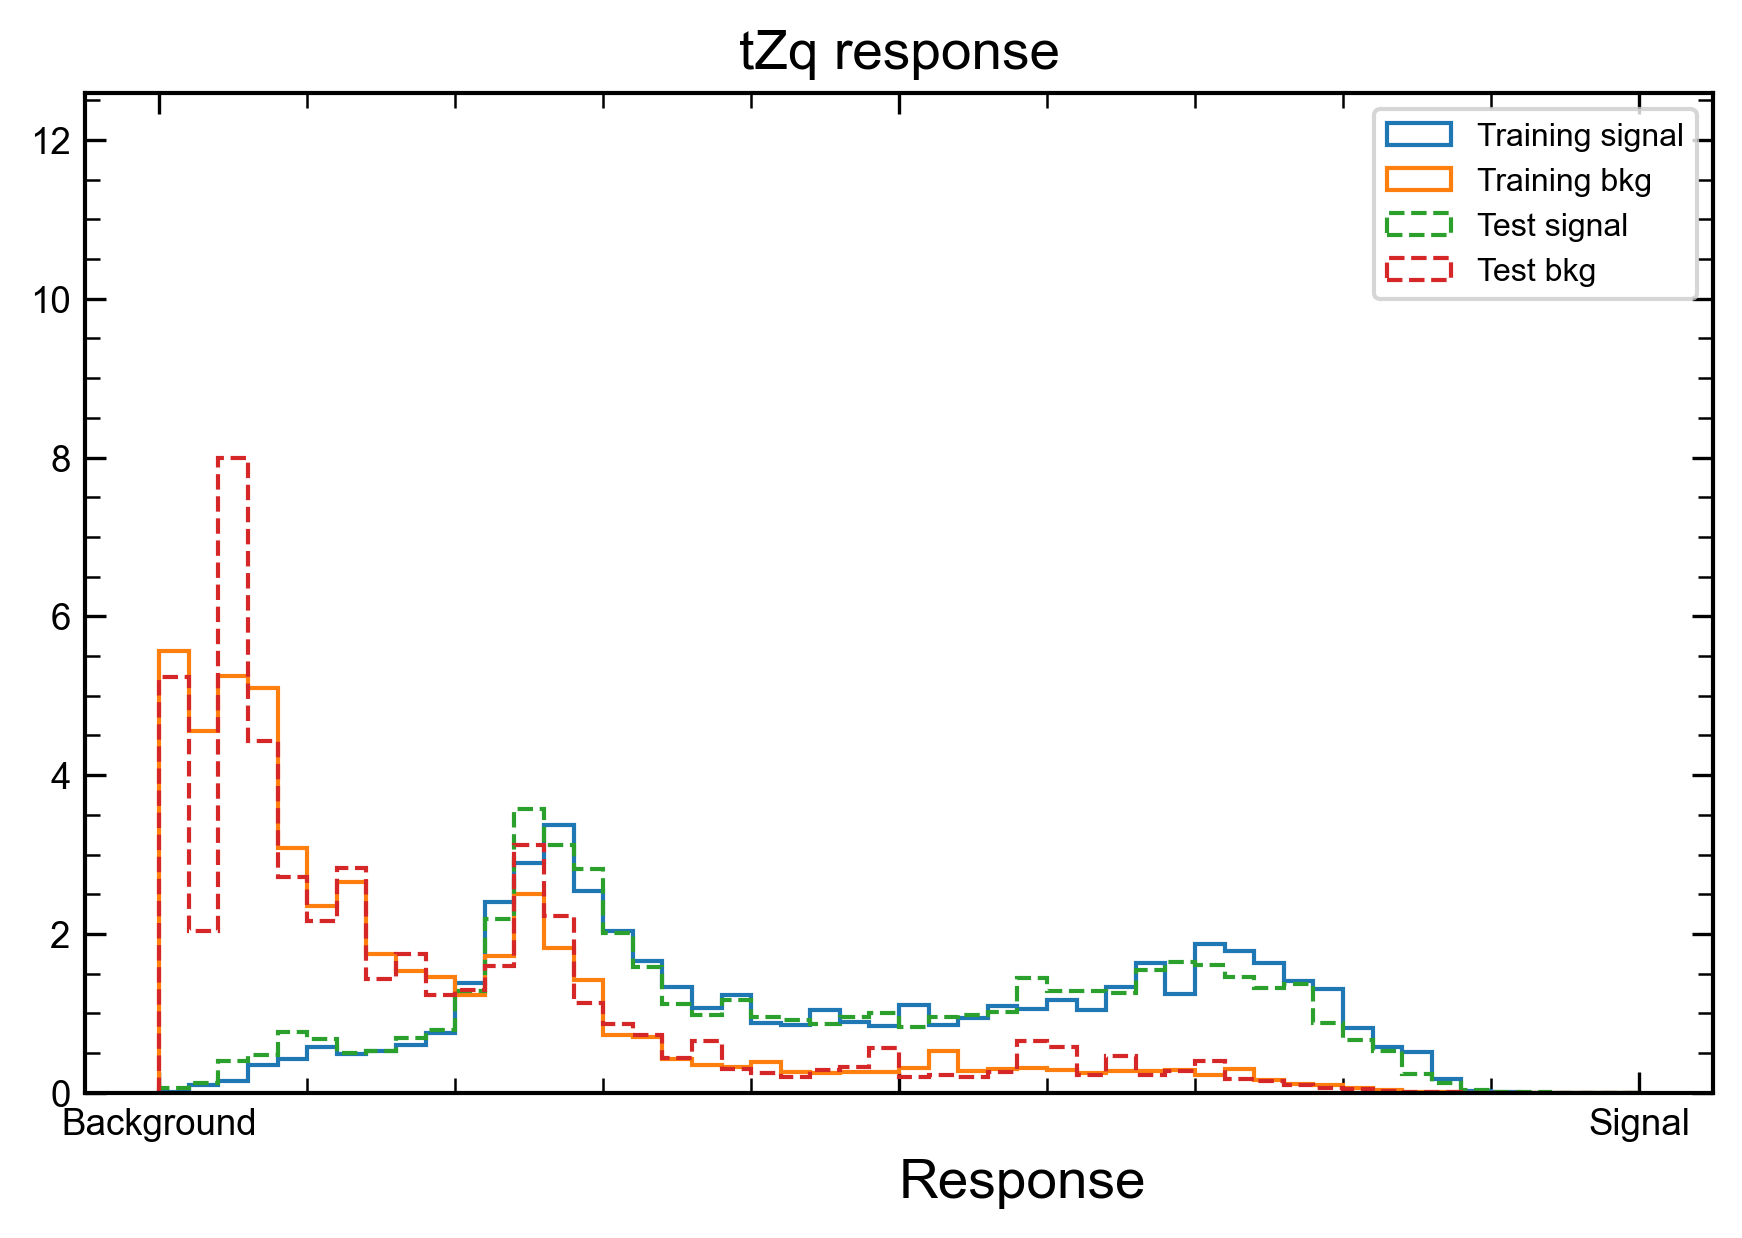
\includegraphics[width=0.8\textwidth]{resp1}
      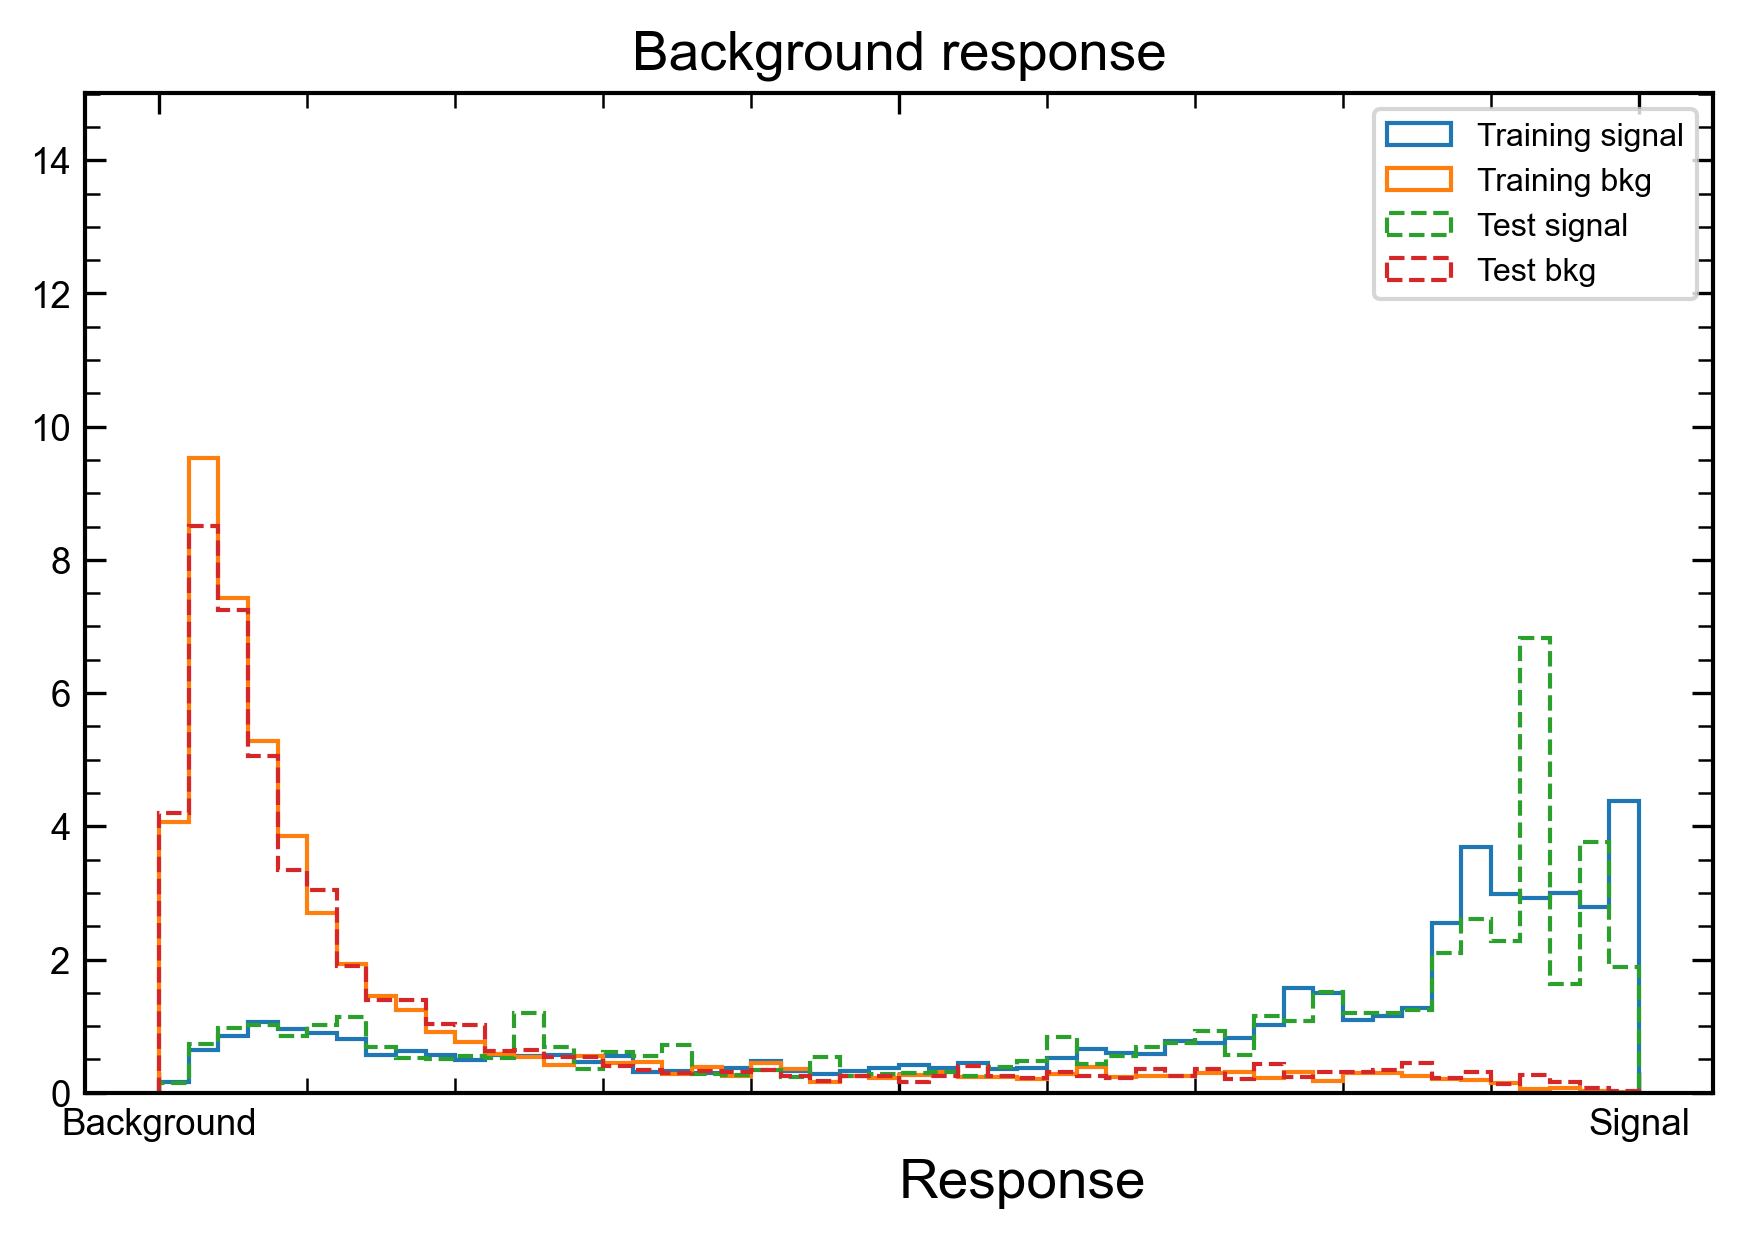
\includegraphics[width=0.8\textwidth]{resp2}
    \end{column}
    \begin{column}{0.5\textwidth}
      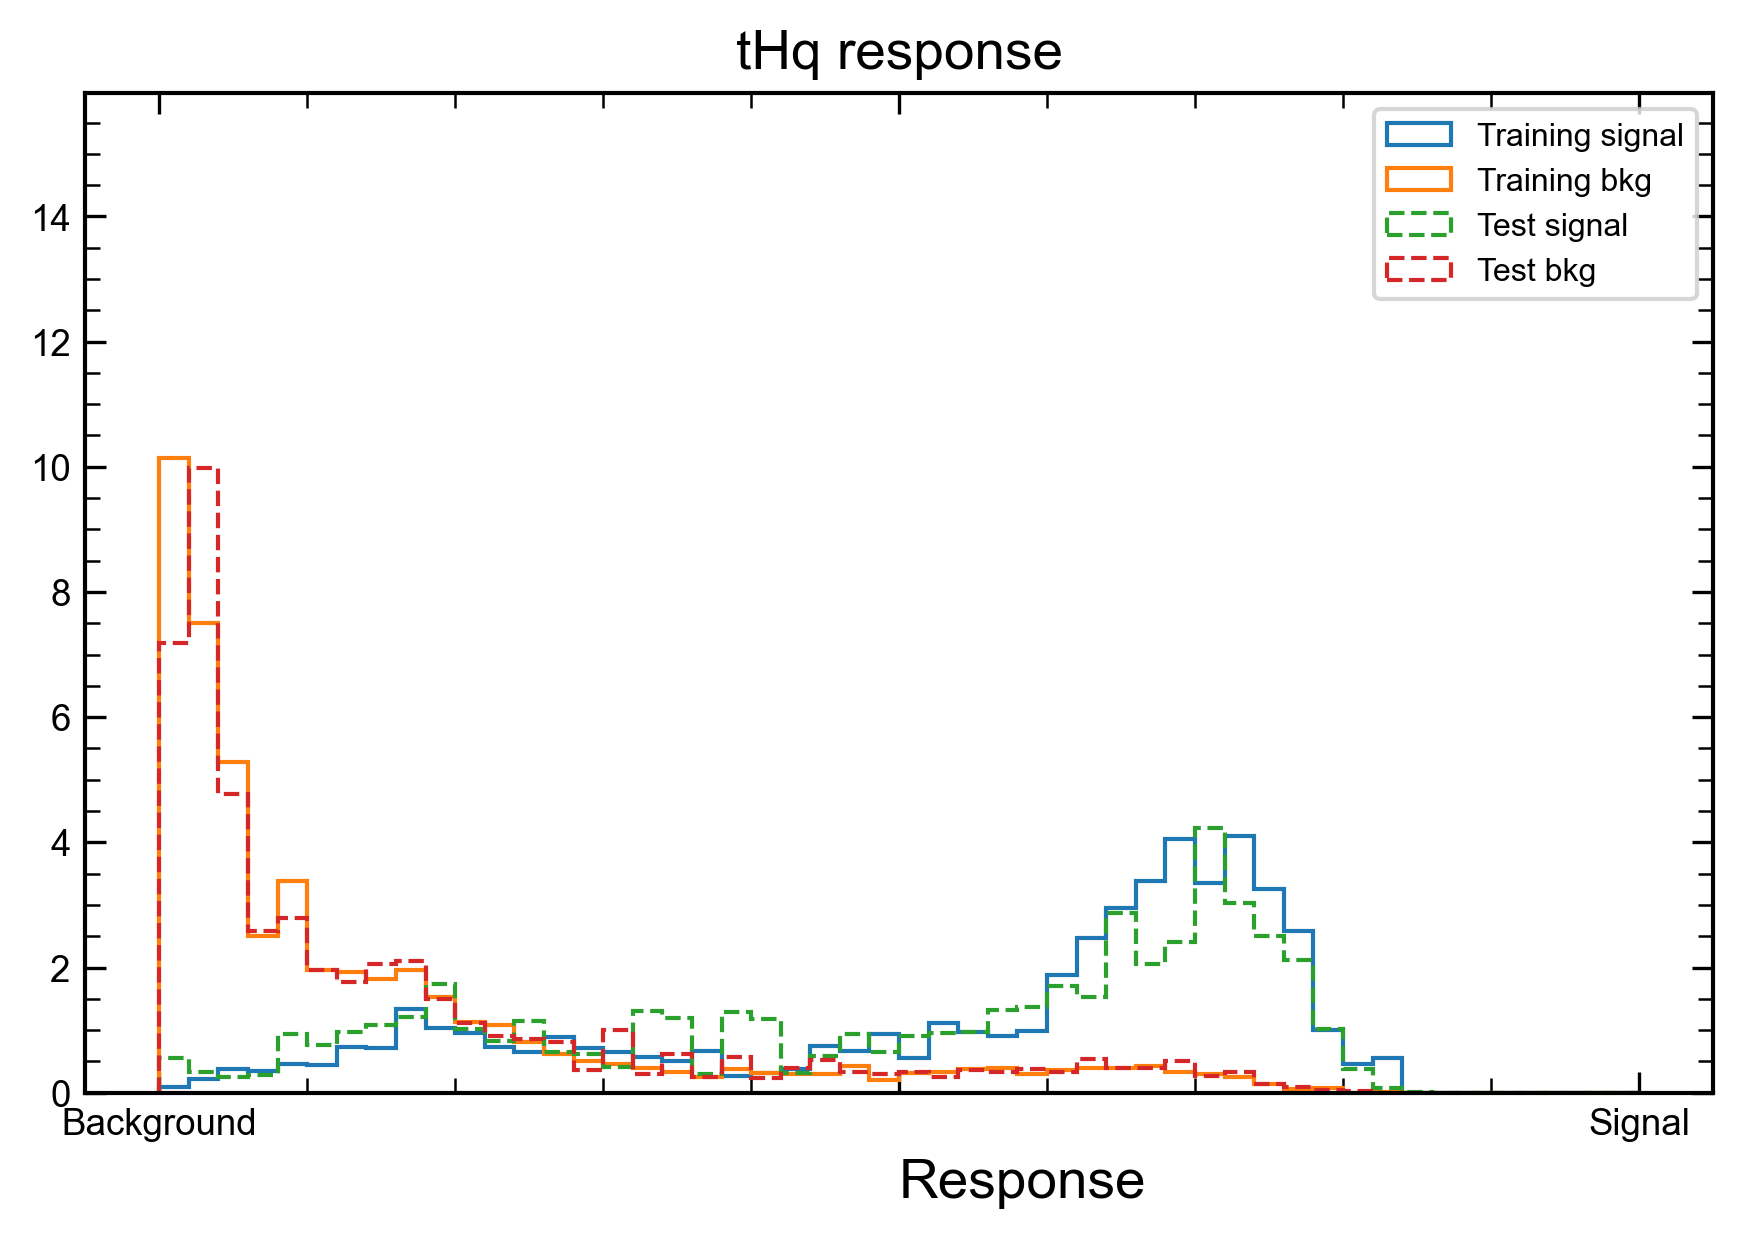
\includegraphics[width=0.8\textwidth]{resp3}
      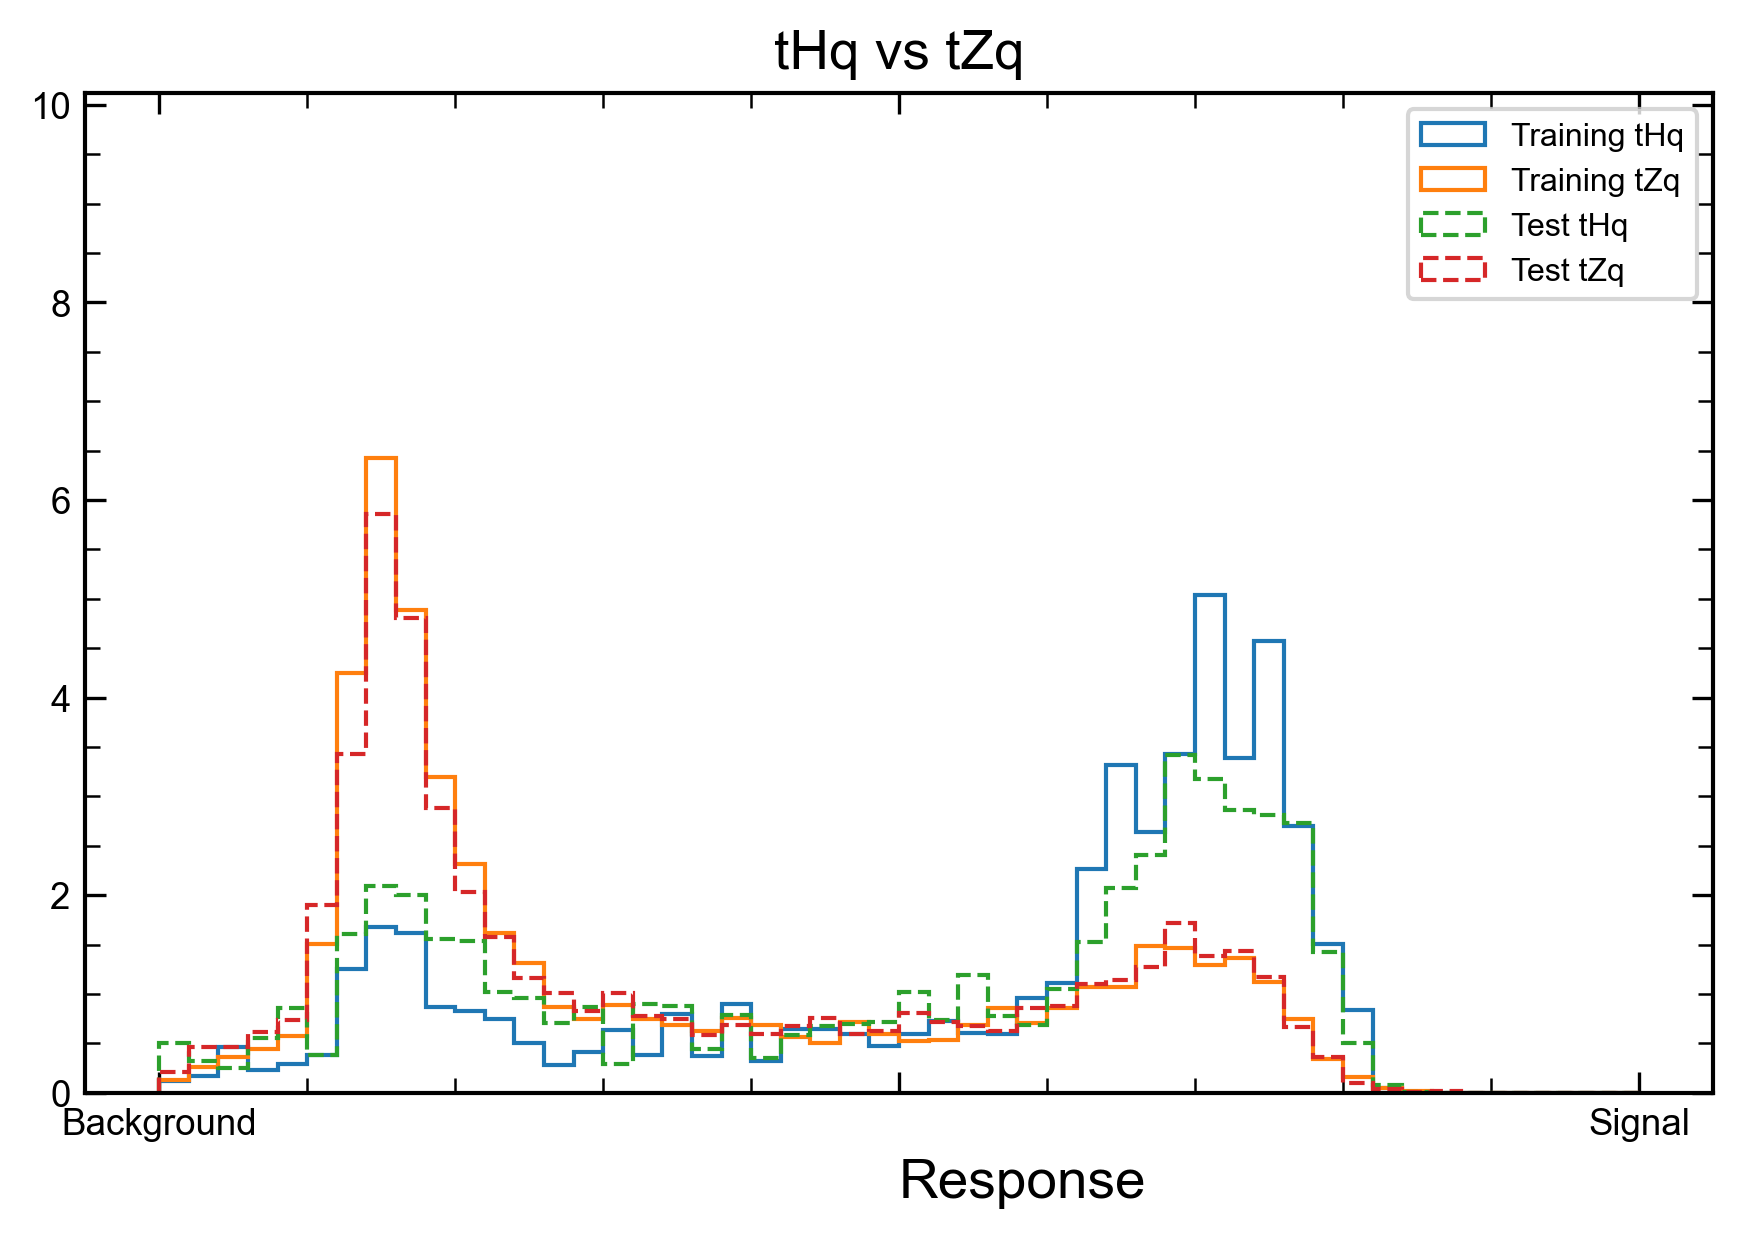
\includegraphics[width=0.8\textwidth]{resp4}
    \end{column}
  \end{columns}    
\end{frame}





\begin{frame}{Conclusion}

\begin{itemize}
  \item \Large No excuses for ignoring other MVA talks
  \vspace{0.5cm}
  \item Categorical neural networks are a promising approach
  \vspace{0.1cm}
  \item More testing and better plots needed
  \vspace{0.1cm}
  \item Testing for more backgrounds easily possible
\end{itemize}
\end{frame}


\begin{frame}{General ML selection}
    \begin{columns}
      \begin{column}{0.5\textwidth}
        \centering 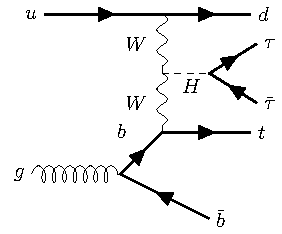
\includegraphics[width=0.8\textwidth]{/cephfs/user/s6chkirf/feynman_diagrams/tHq_tautau}\\
                \begin{itemize}
          \item n-jets: 2 (b-jets: \textbf{1})
          \item b-jet WP: 70 DL1r
          \item nLeptons \& nTaus: $\bf{2e / \mu~1\tau_{\text{had}}} $
          \item $E_{\text{T,miss}}$: no cut (to \SI{800}{GeV})
        \end{itemize}
      \end{column}
      \begin{column}{0.7\textwidth}
        \vspace*{-0.05\textwidth}
        \begin{itemize}
          \footnotesize
          \item jets:
          \vspace*{-0.02\textwidth}
          \begin{itemize}
            \footnotesize
            \item $p_T>\SI{35}{GeV}$
            \item $|\eta|<4.5$
            \item EMPFlow
          \end{itemize}
          \item electrons:
          \vspace*{-0.02\textwidth}
          \begin{itemize}
            \footnotesize
            \item $p_T>\SI{20}{GeV}$ leading \SI{27}{GeV}
            \item $|\eta|<2.5$ not in 1.37 - 1.52
            \item WP: LooseAndBLayerLH ; \\isolation: no requirement
          \end{itemize}
          \item muons:
          \vspace*{-0.02\textwidth}
          \begin{itemize}
            \footnotesize
            \item $p_T>\SI{20}{GeV}$ leading \SI{27}{GeV}
            \item $0.01<|\eta|<2.5$
            \item WP: Loose ; isolation: no requirement
          \end{itemize}
          \item taus:
          \vspace*{-0.02\textwidth}
          \begin{itemize}
            \footnotesize
            \item $p_T>\SI{20}{GeV}$ leading \SI{27}{GeV}
            \item $|\eta|<2.5$ not in 1.37 - 1.52
            \item WP: RNNLoose
            \item ASG recommended OLR ($\tau_{had}$ remove jets)
          \end{itemize}
        \end{itemize}
      \end{column}
    \end{columns}
  \end{frame}
%
%
\begin{frame}{Features and weight setup}
  \begin{itemize}
    \item Absolute weights for training because \rightarrow best and most stable results
    \item Preliminary selection of variables
  \end{itemize}
    \begin{columns}
        \begin{column}{0.5\textwidth}
            \resizebox{\linewidth}{!}{
            \begin{tabular}{|l|l|}
                \hline
                eta\_jf          & forward jet eta                        \\ \hline
                pt\_jf           & forward jet transverse momentum        \\ \hline
                mass\_jf         & forward jet mass                       \\ \hline
                phi\_jf          & forward jet phi                        \\ \hline
                eta\_b           & b-jet eta                              \\ \hline
                pt\_b            & b-jet transverse momentum              \\ \hline
                phi\_b           & b-jet phi                              \\ \hline
                HvisMass         & mass of LorentzV sum of hadronic taus  \\ \hline
                m\_met           & Missing energy                         \\ \hline
                Reco\_w\_mass\_2 & Reconstructed mass of the W case 1     \\ \hline
                Reco\_w\_mass\_1 & Reconstructed mass of the W case 2     \\ \hline
            \end{tabular}}
        \end{column}
        \begin{column}{0.5\textwidth}
            \resizebox{\linewidth}{!}{
            \begin{tabular}{|l|l|}
                 \hline
                 deltaRTau        & Delta R of the hadronic taus          \\ \hline
                 deltaPhiTau      & Delta phi of the hadronic taus        \\ \hline
                 HvisPt           & pt of LorentzV sum of hadronic taus      \\ \hline
                 HvisEta          & eta of LorentzV sum of hadronic taus      \\ \hline
                 TvisMass         & mass of reconstructed top             \\ \hline
                 TvisPt           & pt of visible top                     \\ \hline
                 TvisEta          & eta of visible top                    \\ \hline
                 M\_b\_jf         & Mass of LorentV sum of b and jf       \\ \hline
                 HT               & Sum of transverse energies            \\ \hline
                 lep\_Top\_pt     & Light lepton pt                       \\ \hline
                 lep\_Top\_eta    & Light lepton eta                      \\ \hline
             \end{tabular}}
        \end{column}
    \end{columns}
\end{frame}
  

\end{document}